\documentclass[12pt]{report}
\usepackage{xcolor}
\usepackage[utf8]{inputenc}
\usepackage[numbers]{natbib}%referencing
\usepackage[left=1.0in,right=1.0in,top=.8in,bottom=.8in]{geometry}
\usepackage{float}
\linespread{1.3}
\usepackage{graphicx}%figures
\usepackage{rotating}%landscape
\usepackage{amsmath}%math
\usepackage{amssymb}
\usepackage{titlesec} %formatting chapters
\usepackage{booktabs}
\usepackage{array}
\usepackage{longtable}
\usepackage{multirow}
\usepackage{enumitem}
\usepackage{parskip}
\usepackage{caption}
\usepackage{tikz}
\usepackage{chngcntr}
\usepackage{pgfgantt}
\usepackage{lscape}
\usepackage{hyperref}
\usetikzlibrary{shapes.geometric,arrows.meta,positioning}
%\titlespacing*{<command>}{<left>}{<before-sep>}{<after-sep>}
\titlespacing*{\chapter}{-15pt}{10pt}{15pt}
\titlespacing*{\section}{0pt}{0pt}{5pt}
\titlespacing*{\subsection}{0pt}{5pt}{5pt}
\titleformat{\chapter}[hang]
{\normalfont\huge\bfseries}{\chaptertitlename\ \thechapter.}{1em}{}
\renewcommand{\chaptername}{}
\graphicspath{{Images/}}%image folder name

% Make figures, tables, equations numbered as Chapter.Number
\numberwithin{figure}{chapter}
\numberwithin{table}{chapter}
\renewcommand{\thefigure}{\thechapter.\arabic{figure}}
\renewcommand{\thetable}{\thechapter.\arabic{table}}
\numberwithin{equation}{chapter}

% Hyperref setup
\hypersetup{
    colorlinks=true,
    linkcolor=black,
    urlcolor=black,
    citecolor=black,
    plainpages=false,
    hypertexnames=false
}
\urlstyle{same}

%Cover page contents
\newsavebox{\titlebox}
\begin{lrbox}{\titlebox}
    \begin{minipage}{\textwidth}
        \centering
        
\includegraphics[scale=1.4]{Images/image.png}\\[0.5cm]
        {\large\MakeUppercase{Tribhuvan University}\\
        \MakeUppercase{Institute of Engineering}\\
        \MakeUppercase{National College of Engineering}}\\[0.5cm]
        A Minor Project Report\\
        On\\
        Customer Segmentation and Intelligent Mobile Recommendation System\\[0.5cm]
        \textbf{Submitted By:}\\
        Aayush Chhuka (NCE080BCT002)\\
        Hom Raj Bhandari (NCE080BCT016)\\
        Sudip Kumar Tamang (NCE080BCT042)\\
        Suresh Khadka (NCE080BCT046)\\[0.5cm]
        \textbf{Submitted To:}\\
        Department of Electronics \& Computer Engineering
    \end{minipage}
\end{lrbox}
\title{\usebox{\titlebox}}
\author{}
\date{July, 2026}

\begin{document}
\maketitle
\pagenumbering{roman}
\setcounter{page}{2}
\chapter*{Page of Approval}
\addcontentsline{toc}{chapter}{\numberline{}Page of Approval}
\vspace{1.5cm}
\begin{center}
\uppercase{
Tribhuvan University\\
Institute of Engineering\\
National College of Engineering\\
Department of Electronics and Computer Engineering
    }
    \end{center}
\vspace{.5cm}
The undersigned certifies that they have read and recommended to the Institute of Engineering for acceptance of a project report entitled \textbf{"Customer Segmentation and Intelligent Mobile Recommendation System"} submitted by \textbf{Aayush Chhuka}, \textbf{Hom Raj Bhandari}, \textbf{Sudip Kumar Tamang}, \textbf{Suresh Khadka} in partial fulfillment of the requirements for the Bachelor's degree in Electronics, Information and Communication Engineering \& Computer Engineering.

\vspace{1cm}
\begin{minipage}{.5\textwidth}
        \raggedright
    .............................\\
    Supervisor\\
    \textbf{Mr. Subash Pandey}\\
    Department of Electronics and Computer Engineering,\\
    National College of Engineering, IOE, TU.\\
    \end{minipage}%
    \begin{minipage}{0.5\textwidth}
    \raggedleft
    \hspace{2cm}.............................\\
    \hspace{2cm}External examiner\\
    \hspace{2cm}\textbf{Full Name}\\
    \hspace{2cm}Designation\\
    \hspace{2cm}Affiliation
    \end{minipage}\\
 \newline
 \newline
 \newline
\centerline{Date of approval:}

%new chapter
\chapter*{Copyright}
\addcontentsline{toc}{chapter}{\numberline{}Copyright}
The author has agreed that the Library, Department of Electronics and Computer Engineering, National College of Engineering, and Institute of Engineering may make this report freely available for inspection. Moreover, the author has agreed that permission for extensive copying of this project report for scholarly purposes may be granted by the supervisors who supervised the work recorded herein or, in their absence, by the Head of the Department wherein the project report was done. It is understood that recognition will be given to the author of this report and the Department of Electronics and Computer Engineering, National College of Engineering, IOE for any use of the material of this project report. Copying publication or the other use of this report for financial gain without the approval of to the Department of Electronics and Computer Engineering, National College of Engineering, Institute of Engineering, and the author's written permission is prohibited.

Request for permission to copy or to make any other use of the material in this report in whole or in part should be addressed to:\\
\newline
\newline
\newline
Head\\
Department of Electronics and Computer Engineering\\
National College of Engineering\\
Talchhikhel, Lalitpur.

%new chapter
\chapter*{Acknowledgements}
\addcontentsline{toc}{chapter}{\numberline{}Acknowledgements}
We would like to express our sincere gratitude to the Department of Electronics and Computer Engineering at National College of Engineering for providing us with the opportunity, facilities, and support needed to complete this minor project. The guidance and learning environment provided by the department helped us throughout the development of this project.

We would like to sincerely thank our project supervisor, Mr. Subash Pandey, for his continuous guidance, valuable suggestions, and patient support during every stage of the project. His feedback helped us improve our work and solve many technical and practical problems. His encouragement motivated us to complete the project with confidence.

Finally, we express our heartfelt thanks to our families, friends, and classmates for their constant encouragement, patience, and moral support throughout this journey. We are thankful to everyone who directly or indirectly contributed to the successful completion of this minor project.

\vspace{1cm}
\noindent
Aayush Chhuka (NCE080BCT002) \\
Hom Raj Bhandari (NCE080BCT016) \\
Sudip Kumar Tamang (NCE080BCT042) \\
Suresh Khadka (NCE080BCT046)

%new chapter
\chapter*{Abstract}
\addcontentsline{toc}{chapter}{\numberline{}Abstract}
The mobile phone market offers a wide range of smartphones with different prices, features, and specifications, making it difficult for customers to choose a suitable device and for retailers to understand customer preferences. This project presents a machine learning based customer segmentation and intelligent mobile recommendation system that addresses this challenge by combining smartphone specification data with customer transaction behaviour.

The system uses the XGBoost algorithm, a powerful gradient boosting technique for structured data, to predict smartphone performance scores from hardware specifications and estimate customer spending behaviour. The trained model achieves an R\textsuperscript{2} score of approximately 0.88 on the held-out test set and a mean absolute error of about 0.18 on the log-transformed target. SHAP (SHapley Additive exPlanations) analysis is performed to identify the most influential customer and smartphone features affecting the predictions.

For customer segmentation, the K-Means clustering algorithm is applied to engineered customer features. The optimal number of clusters is selected using the elbow method and silhouette score, producing meaningful groups such as flagship Apple users, value-conscious Samsung buyers, and frequent browsers with low purchasing activity. Each customer is assigned to a cluster, enabling personalised recommendations and customer personas.

The complete system is implemented as a web application using React for the frontend, Node.js and Express for the backend, Prisma ORM, and PostgreSQL for data management. Authentication is handled using Passport with bcrypt password hashing, while role-based access control provides separate functionalities for customers, sales staff, and administrators. The system integrates XGBoost-based performance prediction, K-Means customer segmentation, and SHAP-based explainability into a single platform.

Keywords: \textit{customer segmentation, mobile recommendation system, XGBoost, K-Means clustering, SHAP}
\tableofcontents
\addcontentsline{toc}{chapter}{\numberline{}Contents}
\listoffigures
\addcontentsline{toc}{chapter}{\numberline{}List of Figures}
\listoftables
\addcontentsline{toc}{chapter}{\numberline{}List of Tables}
\chapter*{List of Abbreviations}
\addcontentsline{toc}{chapter}{\numberline{}List of Abbreviations}
\begin{tabbing}
\hspace{3cm} \= \kill
API \> Application Programming Interface \\
BCT \> Bachelor in Computer Engineering \\
CPU \> Central Processing Unit \\
CSS \> Cascading Style Sheet \\
CSV \> Comma Separated Values \\
DBSCAN \> Density-Based Spatial Clustering of Applications with Noise \\
GPU \> Graphics Processing Unit \\
HTML \> HyperText Markup Language \\
HTTP \> HyperText Transfer Protocol \\
ID \> Identifier \\
JSON \> JavaScript Object Notation \\
LIME \> Local Interpretable Model-agnostic Explanations \\
MAE \> Mean Absolute Error \\
MAPE \> Mean Absolute Percentage Error \\
ML \> Machine Learning \\
MSE \> Mean Squared Error \\
NCE \> National College of Engineering \\
ORM \> Object Relational Mapper \\
OTP \> One Time Password \\
PCA \> Principal Component Analysis \\
RAM \> Random Access Memory \\
REST \> Representational State Transfer \\
RMSE \> Root Mean Squared Error \\
RMSLE \> Root Mean Squared Logarithmic Error \\
SHAP \> SHapley Additive exPlanations \\
SQL \> Structured Query Language \\
UI \> User Interface \\
XAI \> Explainable Artificial Intelligence \\
XGBoost \> Extreme Gradient Boosting \\
\end{tabbing}
\chapter{Introduction}
\pagenumbering{arabic}%start arabic numbering(1,2,3..) from here
\section{Background}
The mobile phone market is one of the most competitive consumer electronics industries in the world. New smartphones are introduced frequently by brands such as Samsung, Apple, Xiaomi, Vivo, Oppo, and Realme, each offering different specifications, prices, and features. As a result, customers often find it difficult to choose a phone that best suits their needs and budget, while mobile retailers face the challenge of understanding customer preferences in order to recommend suitable devices.

Customer segmentation is a widely used marketing technique that groups customers based on shared characteristics such as age, spending behaviour, brand preference, and purchasing habits instead of treating every customer the same way \cite{singh}. Once these groups are identified, retailers can provide personalised recommendations, targeted promotions, and better inventory planning. This approach is particularly useful in the smartphone market because customers prioritise different features such as performance, camera quality, battery life, brand reputation, and price.

The increasing availability of customer and product data has made intelligent recommendation systems more practical. Online stores record customer interactions, while GSMArena provides detailed smartphone specifications \cite{gsmarena} and AnTuTu publishes benchmark scores that measure device performance \cite{antutu}. Combining these datasets enables recommendations based on both customer behaviour and the actual technical capabilities of smartphones.

However, many recommendation systems rely heavily on previous purchases, browsing history, or ratings, resulting in the well-known cold-start problem, where new customers or newly released phones receive poor recommendations due to limited historical data \cite{pandey}. Smaller retailers also often rely on simple sales reports that fail to capture meaningful differences between customer groups.

This project addresses these challenges in the context of mobile retailers in Nepal, where purchasing decisions are strongly influenced by price, brand trust, and recommendations from sales staff. The proposed system combines a customer transaction dataset containing more than sixteen thousand records with a cleaned smartphone specification dataset of over eight thousand devices collected from GSMArena together with AnTuTu benchmark scores. After preprocessing and feature engineering, these datasets are used to model customer preferences and smartphone characteristics.

The machine learning component uses the XGBoost algorithm, a powerful gradient boosting technique for structured data \cite{chen}. It is used to predict smartphone performance scores from hardware specifications and estimate customer spending behaviour from purchase history. The trained model achieved an R\textsuperscript{2} score of approximately 0.85 with a mean absolute error of about 0.19 on the log-transformed target. SHAP analysis is also performed to identify the most influential customer and smartphone features affecting the model's predictions.

For customer segmentation, the project applies the K-Means clustering algorithm to the engineered customer features. The optimal number of clusters is selected using the elbow method and silhouette score, producing meaningful groups such as flagship Apple users, value-conscious Samsung buyers, and frequent browsers with low purchasing activity. Each customer is assigned to a cluster, allowing the system to generate personalised recommendations and customer personas.

The complete system is implemented as a web application using React for the frontend, Node.js and Express for the backend, Prisma ORM, and PostgreSQL for data management. Authentication is handled using Passport with bcrypt password hashing, while role-based access control provides separate functionalities for customers, sales staff, and administrators.

Overall, the project integrates data collection, preprocessing, feature engineering, machine learning, customer segmentation, and web application development into a single recommendation system. By combining predictive modelling with customer segmentation, the system aims to improve smartphone recommendations, enhance customer satisfaction, and support data-driven decision-making for mobile retailers.

\section{Problem Statement}
The mobile phone market offers a wide range of smartphones with different prices, features, and specifications. This makes it difficult for retailers to understand customer preferences and recommend the most suitable mobile phones. Customer preferences are influenced by factors such as performance requirements, camera quality, battery life, budget, and brand preference, which cannot be accurately identified using basic demographic information alone.

Retailers also face challenges in grouping customers based on their purchasing behaviour and using this information to support product recommendations and marketing decisions. Without an intelligent customer segmentation system, recommendations and promotional activities may not effectively match the interests of different customer groups.

Therefore, there is a need to develop a machine learning based customer segmentation system that can analyse customer and product data, identify meaningful customer groups, and support intelligent mobile phone recommendations.

\section{Aim and Objectives}

The aim of this project is to develop an intelligent mobile recommendation system using machine learning based customer segmentation that recommends suitable smartphones based on customer preferences.

\begin{enumerate}[label=\Roman*.]
    \item To collect and preprocess mobile phone data from GSMArena and AnTuTu benchmark through web scraping.

    \item To develop a secure web application with user authentication and database management.

    \item To build a machine learning model for customer segmentation and integrate the machine learning model with the web application.

    \item To evaluate the performance measure and accuracy of the proposed system.
\end{enumerate}

\section{Scope}

This project focuses on developing a machine learning based customer segmentation and mobile phone recommendation system. It uses mobile phone specifications collected from GSMArena and benchmark scores collected from AnTuTu to build the recommendation model.

The project also includes a web-based application with user authentication and database management. The system integrates customer information with mobile phone specifications to provide personalised mobile phone recommendations.

\chapter{Literature Review}
This chapter presents the related work and related theory of the project. It reviews existing systems and methods to position the current work relative to previous research and identifies the techniques adopted for this project.

\section{Related Work}
Chen and Guestrin introduced XGBoost, a scalable gradient boosting framework designed for efficient learning on structured datasets \cite{chen}. The model constructs an ensemble of decision trees in a sequential manner, where each tree corrects the errors of the previous ones while incorporating regularisation techniques to reduce overfitting. XGBoost also supports parallel computation, handles missing values automatically, and efficiently processes high-dimensional data. Experimental evaluations on multiple benchmark datasets demonstrated that XGBoost consistently achieved higher prediction accuracy and significantly faster training speed than existing gradient boosting implementations. Owing to these advantages, XGBoost has become one of the most widely adopted algorithms in recommendation systems, customer analytics, fraud detection, and predictive modelling. In this project, XGBoost is employed to predict the performance score of mobile phones from their hardware specifications.

Recent studies have combined XGBoost with SHAP (SHapley Additive exPlanations) to build explainable recommendation systems \cite{crosssell}. These studies utilise customer transaction history, demographic information, browsing behaviour, and purchase records to predict customer purchasing decisions using XGBoost. SHAP is then applied to quantify the contribution of every input feature toward the final prediction, allowing both businesses and customers to understand why a recommendation was generated. Experimental results reported that the integration of SHAP significantly improves model transparency without sacrificing predictive performance. The studies concluded that explainable recommendation systems increase user trust, simplify model interpretation, and support better business decision-making. This project adopts a similar explainable AI approach by applying SHAP to interpret the influence of different mobile phone specifications on the predicted performance score.

I\c{s}\i k proposed a hyper-personalised recommendation framework for fashion retail by integrating customer segmentation with recommendation algorithms \cite{isik}. The proposed system first performs customer segmentation using RFM (Recency, Frequency, Monetary) analysis together with K-Means clustering. Customer location information is then incorporated into the segmentation process, while association rules generated using the Apriori algorithm are employed to produce personalised product recommendations. Experimental evaluation showed that incorporating geographical information alongside purchasing behaviour improved recommendation relevance and personalisation compared to conventional segmentation methods. The study demonstrated that combining multiple customer characteristics enables businesses to better understand customer preferences and provide more targeted recommendations. These findings inspired the customer segmentation stage of the proposed recommendation system.

Joung and Kim presented an interpretable machine learning framework for customer segmentation that emphasises feature importance rather than relying solely on demographic characteristics \cite{joung}. Their approach extracts product-related features from customer reviews and purchasing behaviour and performs customer segmentation using machine learning techniques. Experimental results indicated that explainable segmentation generates more meaningful customer groups and provides valuable business insights regarding customer preferences and purchasing patterns. The authors concluded that integrating explainable AI with customer segmentation improves model interpretability and supports strategic marketing decisions. Their work provides the motivation for incorporating explainability into the customer analysis component of this project.

A recent study proposed a SHAP-enhanced customer segmentation framework for retail analytics by combining advanced feature engineering, Principal Component Analysis (PCA), and multiple clustering algorithms \cite{pcadbscan}. The framework compares clustering methods including K-Means, DBSCAN, Agglomerative Clustering, and Gaussian Mixture Models before selecting the best-performing algorithm using clustering evaluation metrics. Experimental results demonstrated that combining dimensionality reduction with explainable clustering improves cluster quality, enhances interpretability, and supports more informed business decisions. The study highlighted that explainable clustering enables organisations to better understand customer behaviour while maintaining high analytical performance.

Value-aware recommendation systems have emerged as an important direction in recommender system research \cite{valueaware}. Unlike traditional recommendation systems that focus only on customer preferences, these approaches simultaneously consider customer lifetime value, purchasing frequency, and revenue contribution during recommendation generation. Customers are segmented according to their business value, after which different recommendation strategies are applied to maximise both customer satisfaction and organisational profitability. Experimental studies reported improvements in customer retention, recommendation effectiveness, and overall business revenue when customer value was incorporated into recommendation strategies. The findings emphasise that recommendation systems should optimise not only recommendation accuracy but also long-term business objectives.

Zhang \textit{et al.} proposed a large-scale purchase prediction framework using customer behavioural data collected from the Tmall Recommendation Prize competition \cite{zhang}. The framework utilises click history, shopping cart activities, purchase records, and user interaction features to predict future purchasing behaviour through ensemble machine learning models. Extensive experiments demonstrated that behavioural features substantially improve purchase prediction accuracy compared with demographic information alone. The authors concluded that customer interaction data provides valuable information for understanding purchasing intentions and significantly enhances recommendation performance in large-scale e-commerce environments. Their work highlights the importance of incorporating behavioural features into recommendation systems.

Several studies in predictive analytics for e-commerce have investigated the effectiveness of customer browsing behaviour, clickstream data, and historical transaction records for predicting future purchasing activities \cite{predictive}. These studies compared traditional machine learning algorithms such as Logistic Regression with ensemble methods including Random Forest, Gradient Boosting, and XGBoost. Experimental results consistently showed that tree-based ensemble models outperform linear models in terms of prediction accuracy, precision, recall, and robustness when handling complex customer behaviour. The research further demonstrated that combining multiple behavioural features enables businesses to identify purchasing intentions more accurately, thereby improving recommendation quality and customer engagement.

Customer segmentation combined with personalised recommendation has become one of the most widely adopted approaches in modern recommender systems \cite{segmentrecommend}. In these systems, customers are first grouped into homogeneous clusters using techniques such as K-Means clustering based on purchasing behaviour, demographic characteristics, or RFM features. Separate recommendation strategies are then developed for each customer segment. Experimental evaluations consistently reported higher recommendation accuracy, improved personalisation, increased customer satisfaction, and better marketing effectiveness compared with traditional recommendation approaches. These findings demonstrate the effectiveness of integrating customer segmentation into recommendation systems.

Recent explainable recommendation frameworks combine recommendation algorithms with explainable AI techniques such as SHAP, LIME, and knowledge graph-based explanations to improve transparency and user trust \cite{xairecommend}. These systems not only generate personalised product recommendations but also provide understandable explanations by identifying the most influential customer and product features responsible for each recommendation. Experimental results indicate that explainable recommendations improve user confidence, increase acceptance of recommendations, and assist businesses in validating model decisions. The studies conclude that explainability is becoming an essential component of modern recommendation systems, particularly in applications where transparency and trust are critical.

The reviewed literature demonstrates that XGBoost provides highly accurate and computationally efficient prediction for structured datasets, making it well suited for recommendation and predictive analytics applications. The integration of SHAP further enhances model transparency by explaining feature contributions without reducing predictive performance. Existing research also shows that customer segmentation using K-Means and RFM analysis significantly improves recommendation relevance by grouping customers with similar purchasing behaviours and preferences. Furthermore, behavioural features such as browsing history, clickstream data, and transaction records consistently improve purchase prediction accuracy, while explainable recommendation techniques increase user trust and business interpretability. These findings collectively provide a strong foundation for the proposed mobile phone recommendation system, which integrates XGBoost-based performance prediction, K-Means customer segmentation, and SHAP-based explainability to deliver accurate, personalised, and interpretable recommendations.

\section{Related Theory}

\subsection{Gradient Boosting}

Gradient Boosting is an ensemble machine learning technique that combines multiple weak decision trees to create a strong predictive model \cite{friedman}. The trees are built one after another, where each new tree learns from the errors made by the previous trees. This sequential learning process improves the overall prediction accuracy and enables the model to capture complex patterns in structured data.

\subsection{XGBoost}

Extreme Gradient Boosting (XGBoost) is an optimised implementation of the Gradient Boosting algorithm \cite{chen}. It is widely used because of its high accuracy, fast training speed, and ability to handle large tabular datasets. XGBoost includes built-in regularisation to reduce overfitting, automatically handles missing values, and efficiently works with both numerical and categorical features after appropriate encoding. These characteristics make it well suited for customer segmentation, recommendation, and prediction tasks involving mobile phone specifications and customer transaction data.

In this project, XGBoost is used as the primary machine learning algorithm to predict mobile phone performance scores and support the recommendation system.

\subsection{SHAP (SHapley Additive exPlanations)}

SHAP (SHapley Additive exPlanations) is an Explainable Artificial Intelligence (XAI) technique used to interpret machine learning models \cite{lundberg}. It explains how each input feature contributes to a model's prediction by assigning an importance value, called the SHAP value, to every feature. Positive SHAP values indicate that a feature increases the prediction, while negative values indicate that it decreases the prediction.

SHAP provides both global explanations, which show the overall importance of features across the entire dataset, and local explanations, which explain the prediction for an individual sample. This makes it easier to understand the behaviour of complex models such as XGBoost.

In this project, SHAP is used to explain the predictions made by the XGBoost model by identifying the most influential phone specifications responsible for the predicted performance score.

\subsection{K-Means Clustering}

K-Means Clustering is an unsupervised machine learning algorithm used to group similar data points into a fixed number of clusters (K) \cite{macqueen}. It works by randomly selecting K cluster centres (centroids), assigning each data point to the nearest centroid, and then updating the centroids based on the mean of the assigned points. This process repeats until the cluster assignments no longer change or a maximum number of iterations is reached. K-Means is simple, efficient, and widely used for customer segmentation, pattern recognition, and data analysis.

\chapter{Methodology}
This chapter presents the methodology and theoretical background of the proposed system. It covers the data sources used, the preprocessing techniques applied, the machine learning algorithms selected with their underlying concepts, and the evaluation metrics used to measure the performance of the trained models.

\section{System Flowchart}

\begin{figure}[H]
\centering
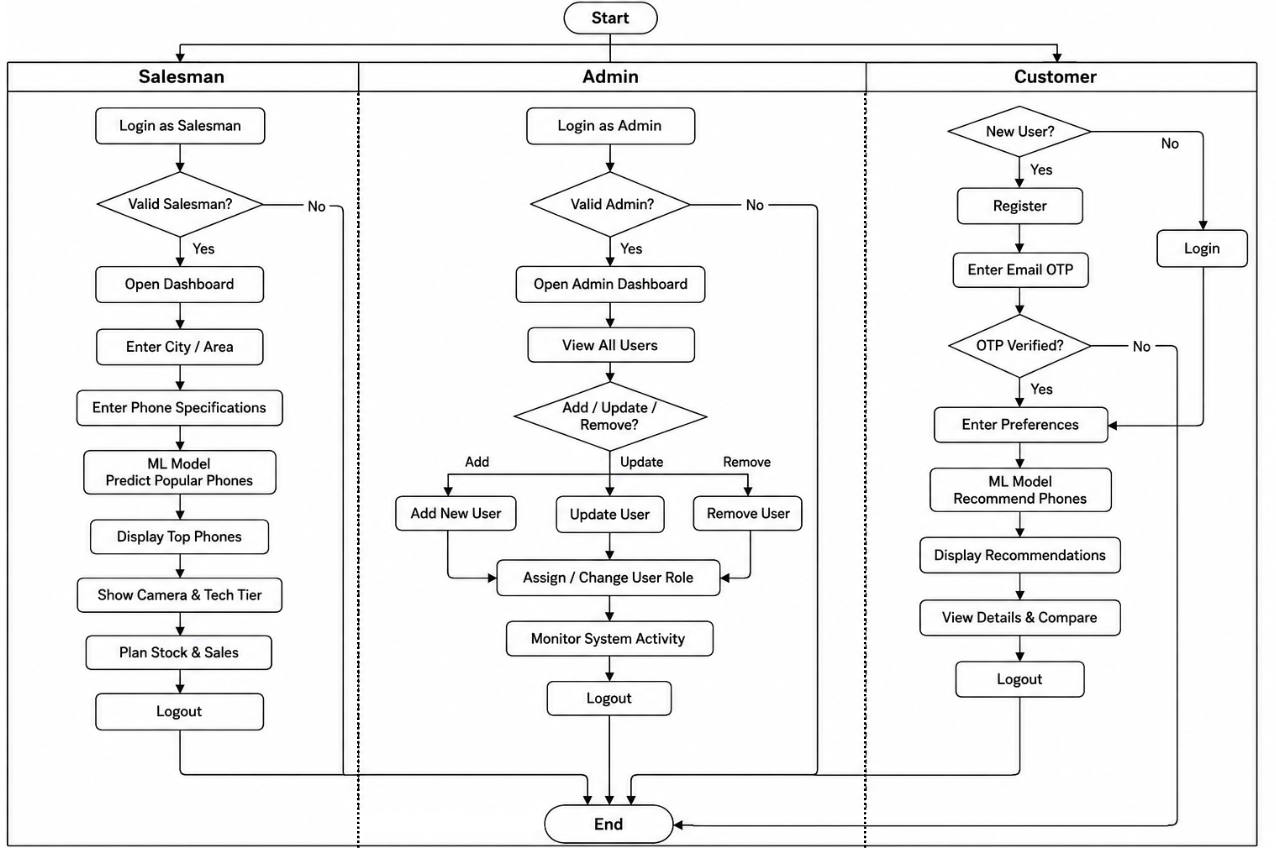
\includegraphics[width=1.0\textwidth]{Images/SystemFlowchart.png}
\caption{System Workflow Flowchart}
\label{fig:systemflow}
\end{figure}
The system flowchart shows the complete path that each user group follows from the moment they enter the system to the moment they leave. The flow starts at the top with a single start node, and then branches into three separate lanes for three different roles. One lane is for the admin, one lane is for the salesman, and one lane is for the customer.

\textbf{Admin Lane:} The admin begins by entering the login screen. The system checks whether the login is valid. If the login is correct, the admin opens the admin dashboard and views the list of all users in the system. The admin then chooses one of three actions: add a new user, update an existing user, or remove a user from the system. After the action is done, the flow comes back to a single step where the admin can assign or change the role of any user. Once the user management work is done, the admin can move to the system monitoring step to check the overall activity in the system. Finally, the admin logs out and the flow reaches the end node. If the login is not valid, the flow also reaches the end node.

\textbf{Salesman Lane:} The salesman begins by entering the login screen. The system checks whether the login is valid. If the login is correct, the salesman opens the salesman dashboard. The salesman then enters required details. This input is passed to the machine learning model, which predicts the suitable phone. The system displays the top phones along with their camera tier and tech tier details. The salesman uses these results to plan which phones to keep in stock and which customers to target. Finally, the salesman logs out and the flow reaches the end node. If the login is not valid, the flow also reaches the end node.

\textbf{Customer Lane:} The customer is first asked whether they are a new user or a returning user. New users are sent to the registration step, where they enter their name, email, and password. A six-digit code is then sent to their email, and the customer enters this code in the system. The system checks whether the code is correct. If the code is verified, the customer moves to the preference step. If the code is not correct, the flow reaches the end node. Returning users skip the registration step and go straight to the login step. From the preference step onwards, both new and returning customers enter their preferences. The machine learning model then recommends matching phones, and the customer views the recommended phones along with their full details. The customer can compare the options and then log out. After the logout, the flow reaches the end node.

\section{Block Diagram of the System}

\begin{figure}[H]
\centering
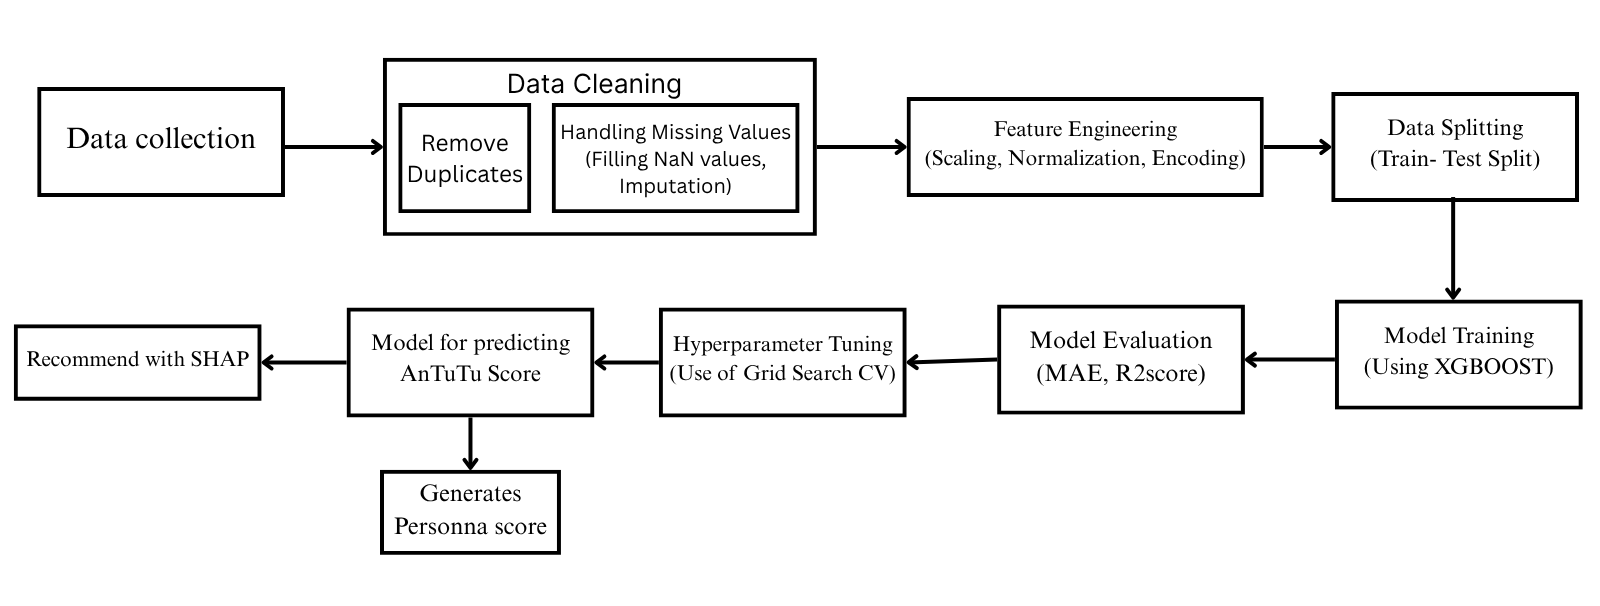
\includegraphics[width=1\textwidth]{Images/pipeline.png}
\caption{Block diagram of the System}
\label{fig:sysarch}
\end{figure}
The pipeline begins by collecting mobile phone specifications, AnTuTu benchmark scores, and customer data. After cleaning and preprocessing the data, an XGBoost regression model is trained to predict the performance score of a phone from its specifications. The model is evaluated and optimised using Grid Search with Cross-Validation. Finally, the predicted performance scores are used in the recommendation system, and SHAP is applied to explain which phone features have the greatest impact on the predictions.

\subsection{Data Collection}

The proposed system requires two categories of input. The first is a dataset of mobile phone specifications, which allows the system to describe every phone that it can recommend. The second is a dataset of customer transactions, which allows the system to model the behaviour of the customers who use the platform. Both datasets are stored in a tabular form and are made available to the training pipeline before any model fitting begins.

\begin{figure}[H]
\centering
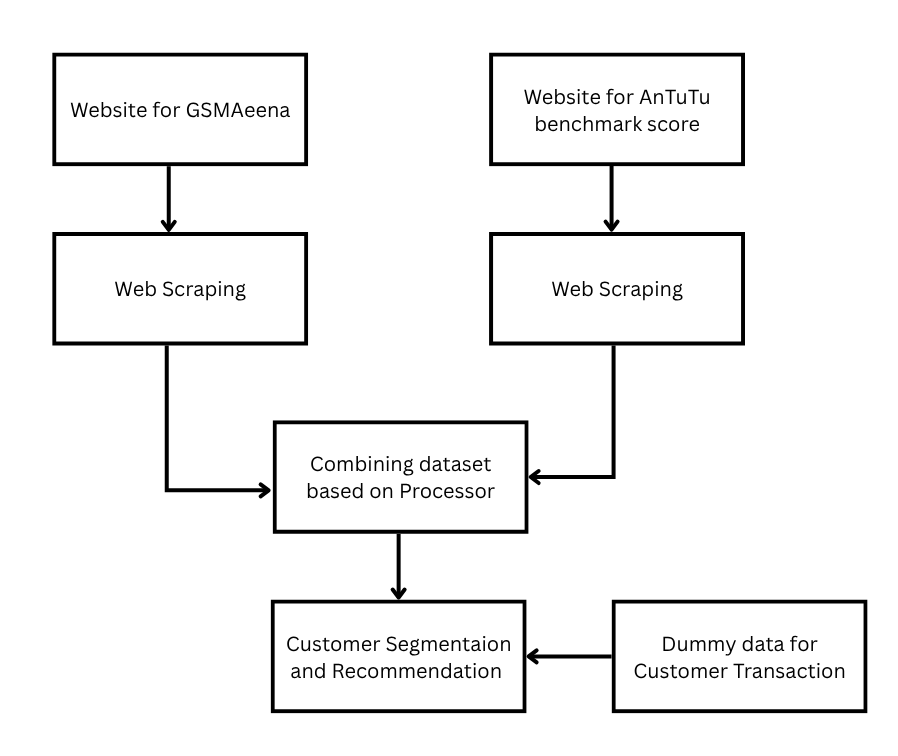
\includegraphics[width=0.95\textwidth]{Images/datacollection.png}
\caption{Data Collection and Integration Process}
\label{fig:datacollection}
\end{figure}

\subsubsection{Phone Specifications}

The phone specification dataset is collected from a public mobile phone database called GSMArena that lists the technical details of mobile phones released over the last several years. The source is selected because it is one of the most complete and consistent public catalogues of mobile phone specifications, and because its schema aligns closely with the fields that the recommendation engine needs. For every phone, the source provides around a hundred fields covering the network technology, the body dimensions, the display, the platform, the memory, the camera, the connectivity, the battery, and the miscellaneous features. The source also provides the model identifier and the model image, both of which are useful for presenting the phone in the user interface. Because the size of the full catalogue is large, the scraping is divided into a number of smaller batches that are run one at a time, so that the public source is not overloaded. The batches are then merged into a single raw dataset that forms the input to the preprocessing stage.

\subsubsection{Benchmark Scores}

A second public source is used to collect benchmark scores for mobile phones. The chosen source is one of the few public aggregators that list benchmark scores for nearly every released phone on a single page. The AnTuTu benchmark is selected because it is one of the most widely cited indicators of overall mobile performance, and because it is available for almost every modern phone. The scraped benchmark table contains the model identifier, the benchmark value, and a uniform resource locator that traces the source of the score. The benchmark values are then merged with the phone specification dataset by matching on a cleaned version of the model identifier. The merged dataset contains the full specification row set with the benchmark score added wherever it is known, and a missing value wherever it is not. The merged file is the input to the model training stage, but only the rows that have a real benchmark value are used for fitting, because using an imputed benchmark as a training target would introduce a circular dependency.

\subsubsection{Customer Transaction Data}

The customer side of the system uses a separate dataset of customer transactions. The transactions describe individual purchases made by customers and are intended to simulate the kind of data that a mobile phone retailer would collect from a real point of sale. The dataset contains one row per transaction and includes information about the customer, the product purchased, the transaction value, the payment method, the time of the transaction, the customer's expressed preferences, and a few derived indicators of loyalty. Because the same customer can have many transactions, the rows are first aggregated to one row per customer before any modelling is performed. The dataset is synthetic and is generated specifically for the project, which makes it possible to demonstrate the segmentation pipeline on data with realistic noise without relying on private customer data.

\section{Data Preprocessing}

The preprocessing stage transforms the raw data into a clean, model-ready form. The transformation is performed in two streams, one for the phone specification data and one for the customer transaction data. The operations performed in each stream are described in the order in which they are applied, together with the reason for each operation.

\begin{figure}[H]
\centering
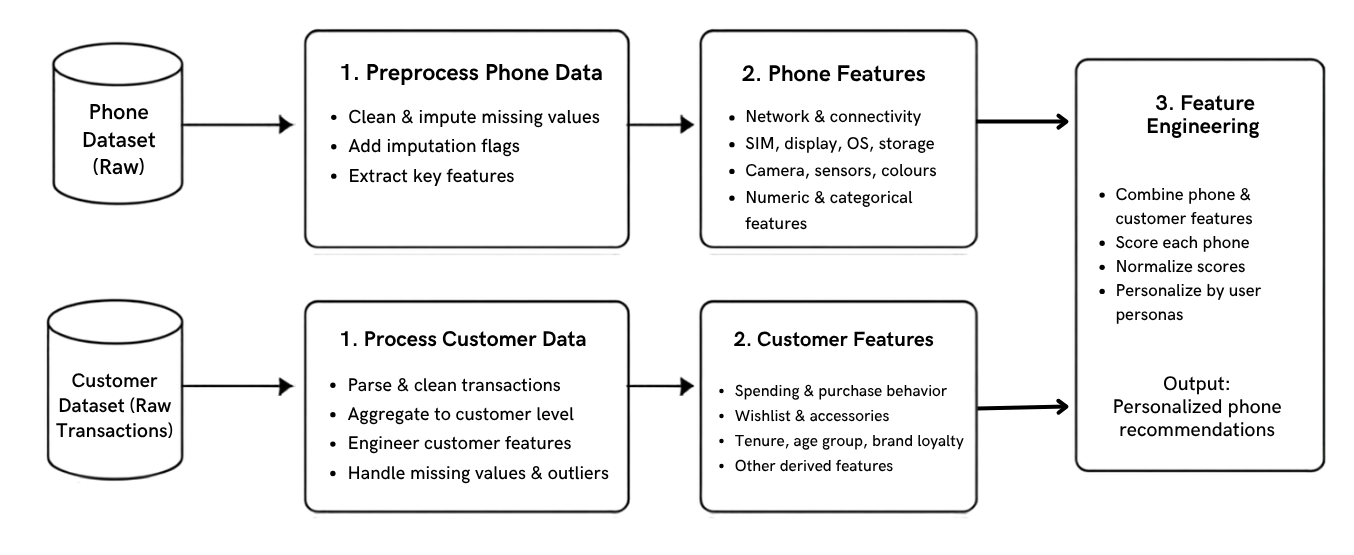
\includegraphics[width=1\textwidth]{Images/dataprocessing.png}
\caption{Data Processing Flow}
\label{fig:dataprocessing}
\end{figure}

\subsection{Phone Dataset Preprocessing}

The CPU, chipset, and GPU columns are converted from free text into structured features. CPU cores, clock speed, architecture, chipset details, GPU vendor, and GPU family are extracted. Missing chipset and GPU values are filled using similar devices based on CPU, chipset, brand, and release year.

Important numeric columns are filled using a three-level median imputation strategy. For selected fields, imputation flags are added to indicate whether the original value was missing.

The network, status, and dimensions columns are transformed into numeric features. Network generation and 5G support are identified, release year and availability are extracted, and device dimensions are used to calculate volume, aspect ratio, and density.

The SIM, display, operating system, and storage columns are converted into compact categorical and binary features. These include SIM type, display technologies, OS version, software support, storage family, and storage performance tier.

The camera, Wi-Fi, GPS, sensors, colours, and FM radio columns are also processed into structured features. Camera capabilities, wireless connectivity, available sensors, and colour count are extracted, while very rare features are removed.

Finally, all original free-text columns are dropped after feature extraction. The final dataset contains only numeric, binary, and low-cardinality categorical features suitable for machine learning models.

\subsection{Customer Dataset Preprocessing}

The customer preprocessing stage converts transaction-level records into a customer-level dataset. List-based columns such as browsing history, wishlist, accessories purchased, and exchange history are first parsed into structured data after correcting boolean values.

The transaction records are then grouped by customer to calculate summary statistics. These include purchase count, total and average spending, purchase frequency, ratings, recency, first and last purchase dates, preferred categories, wishlist and accessory information, exchange count, and brand loyalty.

Additional customer features are created after aggregation. These include customer tenure, wishlist conversion rate, average accessory price, price sensitivity, and age group.

Finally, the aggregated dataset is checked for missing values and outliers. A few derived columns are filled using median values when necessary, while outlier flags are added for spending-related features without removing any records.

\subsection{Feature Engineering}
The cleaned phone dataset undergoes a second stage of feature engineering to create nine user-oriented scores on a 0--100 scale. These scores represent gaming, camera, battery, display, software, security, connectivity, portability, and storage performance using weighted combinations of relevant hardware and software features.

An overall phone score is calculated as the weighted sum of the nine dimension scores. A value score is also computed by comparing the overall score with the phone's price, helping identify devices that offer better value for money.

To ensure consistent scoring, all numeric features are normalised using clipping and logarithmic normalisation methods. The same normalisation parameters are reused during prediction to maintain consistency.

Finally, several user personas such as Gamer, Camera Lover, Battery Focused, All-rounder, and Business User are defined using different weight combinations. A custom persona is also supported, allowing users to assign their own importance ratings to each dimension for personalised recommendations.

\subsection{Scaling, Outlier Handling, and Train Test Preparation}

The regressor used in this project is a tree based model, which is invariant to monotone transformations of the input. For this reason no separate scaling step is applied to the raw features. Outliers are handled implicitly through the first and ninety-ninth percentile clip in the two normalisation helpers, which keeps the composite scores inside a sensible range. Categorical columns are cast to a native categorical type with the training categories frozen at training time, which lets the tree-based model treat them natively and avoid the dummy variable explosion. The training, validation, and test split is an 80/20 random split with a fixed random seed, followed by a 5 fold cross-validation using the same seed. The regressor is trained on rows where the benchmark score was measured rather than imputed, which gives a training set of measured rather than synthesised values.

\section{Methods and Algorithms}

The machine learning stack has two parts. The first is a phone level regression model that scores a phone on nine dimensions and predicts the benchmark value for new phones. The second is a customer level clustering model that groups customers into segments based on their purchase history. A weighted scoring ranker sits on top of the phone model and produces the recommendations.

\subsection{XGBoost Algorithm}

The phone prediction model uses an Extreme Gradient Boosting (XGBoost) regressor to estimate the benchmark score from the processed phone features. The target benchmark score is transformed using $\log(1+x)$ to reduce skewness and improve prediction accuracy, especially for high-end flagship devices. The model is trained using the fixed hyperparameters listed in Table~\ref{tab:xgb-hyperparams}.

\textbf{Mathematical formulation:}
Extreme gradient boosting is a regularised ensemble of $K$ additive decision trees, with the objective

\begin{equation}
\mathcal{L}(\theta) \;=\; \sum_{i=1}^{n} l\!\left(y_i, \hat{y}_i\right) \;+\; \sum_{k=1}^{K} \Omega(f_k)
\label{eq:xgb-objective}
\end{equation}

\noindent where $l$ is the squared error loss on the log transformed target, $f_k$ is the $k$-th tree, and $\Omega$ is a regularisation term. The regularisation used in extreme gradient boosting is

\begin{equation}
\Omega(f) \;=\; \gamma T \;+\; \tfrac{1}{2}\, \lambda \sum_{j=1}^{T} w_j^{2}
\label{eq:xgb-regularisation}
\end{equation}

\noindent where $T$ is the number of leaves in the tree, $w_j$ is the score assigned to leaf $j$, $\gamma$ is the complexity penalty per leaf, and $\lambda$ is the L2 weight decay.

At each boosting round the model fits a new tree to the negative gradient of the loss with respect to the current prediction, and uses the second order Taylor expansion of the loss to pick the best split. For a candidate split that sends $I_L$ samples to the left and $I_R$ samples to the right, the gain is

\begin{equation}
\mathcal{G}_{\text{split}} \;=\; \tfrac{1}{2}\!\left[ \frac{G_L^{2}}{H_L + \lambda} + \frac{G_R^{2}}{H_R + \lambda} - \frac{(G_L + G_R)^{2}}{H_L + H_R + \lambda} \right] \;-\; \gamma
\label{eq:xgb-gain}
\end{equation}

\noindent where $G$ and $H$ are the sums of the first and second order gradients in the node. The split with the largest gain is chosen.

\textbf{Reason for using extreme gradient boosting for this project:} The phone data is mostly tabular, mostly numeric, and contains both continuous values and categorical values. The model handles both kinds of feature without one hot encoding, captures non-linear interactions between features, and is resistant to monotone feature transforms so the logarithmic target and the clipped scores do not need extra preprocessing. The cross-validated coefficient of determination and the test coefficient of determination confirm that the regularised ensemble generalises well beyond the training rows.

\begin{figure}[H]
\centering
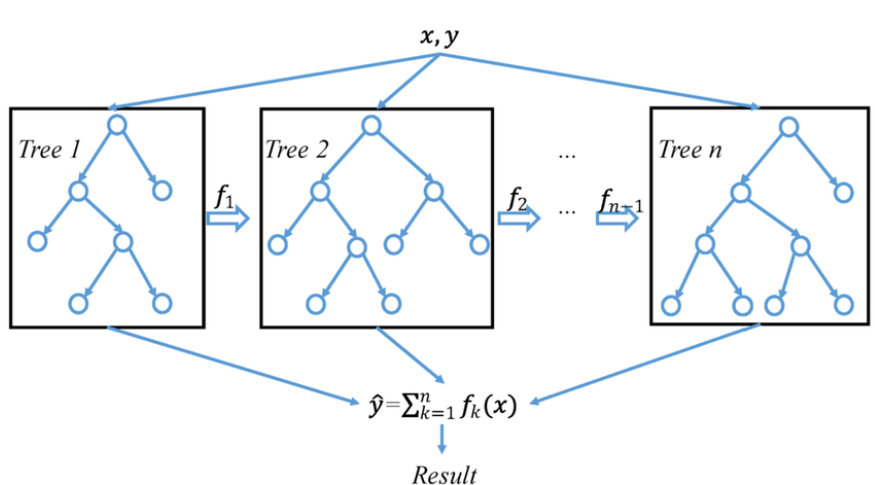
\includegraphics[width=0.8\textwidth]{Images/xgboost.png}
\caption{XGBoost Ensemble of Decision Trees \cite{xgboostimg}}
\label{fig:xgboost}
\end{figure}

\subsection{K-Means Clustering for Customer Segmentation}

Customer segmentation uses the K-Means algorithm on a customer by feature matrix. Twenty numeric features and six categorical features are fed into a column transformer that imputes missing numerics with the median, standardises them with a standard scaler, imputes missing categoricals with the most frequent value, and one hot encodes them with a one hot encoder that drops the first category and ignores unknown categories. The resulting matrix has 64 columns. K-Means is fit with a large number of initialisations and a fixed random seed so the result is reproducible.

\textbf{Mathematical formulation:} K-Means partitions $N$ points into $K$ clusters by minimising the within cluster sum of squared distances,

\begin{equation}
J \;=\; \sum_{k=1}^{K} \sum_{x \in C_k} \lVert x - \mu_k \rVert^{2}
\label{eq:kmeans-objective}
\end{equation}

\noindent where $\mu_k$ is the centroid of cluster $C_k$. Lloyd's algorithm alternates between assigning each point to the nearest centroid and recomputing the centroid of each cluster, and converges to a local minimum of $J$.

\textbf{Number of clusters.} The number of clusters is selected by running K-Means for a range of values of $k$ and recording four metrics: the inertia, the silhouette score, the Davies-Bouldin index, and the Calinski-Harabasz index. The chosen $k$ is the one with the highest Calinski-Harabasz score, subject to a minimum cluster share so that no segment is too small to be useful in a marketing campaign, and to a minimum number of clusters. Agglomerative clustering with Ward linkage and density based spatial clustering are also run on the same data as a cross check, and the agreement of the two methods on the broad shape of the segmentation is used as additional evidence for the choice of $k$.

\textbf{Reason to use K-Means for this project:} The customer data is mostly continuous and the K-Means assumption of roughly spherical clusters is reasonable after the standardisation. K-Means is also the cheapest clustering algorithm to refit when new transaction rows arrive, and the trained model is small enough to be persisted as a single file.

\begin{figure}[H]
\centering
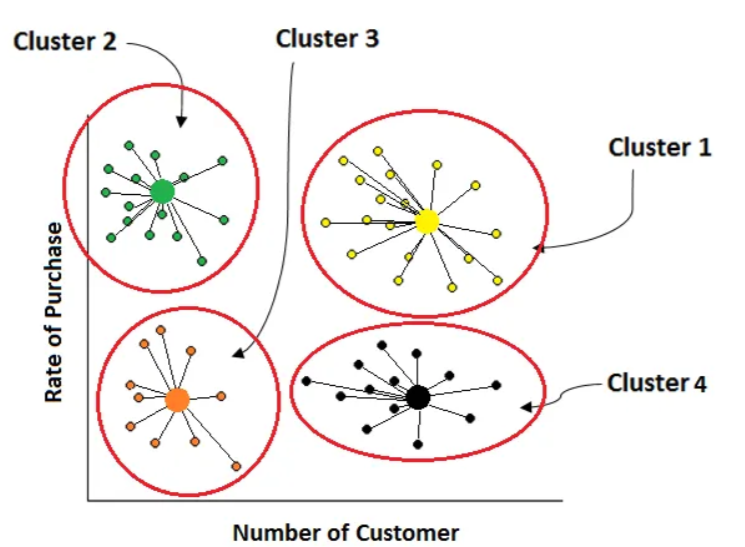
\includegraphics[width=0.8\textwidth]{Images/kmeans.png}
\caption{K-Means Clustering of Customers \cite{kmeansimg}}
\label{fig:kmeans}
\end{figure}

\section{Evaluation Metrics}

The project uses three families of evaluation metrics. The first family is for the regressor that predicts the benchmark score. The second family is for the clustering algorithm that produces the customer segments. The third family is for the recommendation engine, which is the ranker that sits on top of the two models.

\subsection{Metrics for the Regressor}

\textbf{Coefficient of determination ($R^{2}$).} The coefficient of determination measures the fraction of variance in the target that the model explains. It is defined as

\begin{equation}
R^{2} \;=\; 1 - \frac{\sum_{i=1}^{n} \left( y_i - \hat{y}_i \right)^{2}}{\sum_{i=1}^{n} \left( y_i - \bar{y} \right)^{2}}
\label{eq:r2}
\end{equation}

\noindent where $y_i$ is the true log transformed benchmark score, $\hat{y}_i$ is the prediction, and $\bar{y}$ is the mean of the true values. A value of 1 means the model explains all of the variance, a value of 0 means it does no better than predicting the mean, and a negative value means it does worse. In this project the coefficient of determination is computed both on the 80\% training set and on the 20\% held out test set, and also averaged over the 5 folds of a cross-validation, to check that the model is not overfitting. The metric is sensitive to the variance of the target, so it is not directly comparable across datasets, but it is a good internal check.

\textbf{Mean absolute error (MAE).} The mean absolute error measures the average absolute deviation of the predictions from the true values, in the same units as the target.

\begin{equation}
\text{MAE} \;=\; \frac{1}{n} \sum_{i=1}^{n} \left| y_i - \hat{y}_i \right|
\label{eq:mae}
\end{equation}

\noindent In this project the mean absolute error is reported in log space because the model is trained on the logarithm of one plus the benchmark score. The metric is robust to outliers, which matters because the benchmark distribution has a long flagship tail.

\textbf{Mean squared error (MSE).} The mean squared error measures the average of the squared differences between the predictions and the true values. It is defined as

\begin{equation}
\text{MSE} \;=\; \frac{1}{n} \sum_{i=1}^{n} \left( y_i - \hat{y}_i \right)^{2}
\label{eq:mse}
\end{equation}

\noindent where $y_i$ is the true log transformed benchmark score and $\hat{y}_i$ is the prediction. Because the errors are squared before averaging, the metric penalises larger errors more heavily than smaller ones, which makes it sensitive to outliers. In this project the mean squared error is reported in log space to remain consistent with the log transformed target on which the model is trained.

\textbf{Root mean squared error (RMSE).} The root mean squared error is the square root of the mean squared error and is expressed in the same units as the target. It is defined as

\begin{equation}
\text{RMSE} \;=\; \sqrt{\frac{1}{n} \sum_{i=1}^{n} \left( y_i - \hat{y}_i \right)^{2}}
\label{eq:rmse}
\end{equation}

\noindent where $y_i$ is the true log transformed benchmark score and $\hat{y}_i$ is the prediction. Taking the square root restores the original units of the target, which makes the root mean squared error directly comparable to the mean absolute error for the same target. In this project the root mean squared error is reported in log space so that the magnitude of the typical error can be compared with the mean absolute error.

\textbf{Mean absolute percentage error (MAPE).} The mean absolute percentage error expresses the average absolute deviation of the predictions from the true values as a percentage of the true value. It is defined as

\begin{equation}
\text{MAPE} \;=\; \frac{1}{n} \sum_{i=1}^{n} \left| \frac{y_i - \hat{y}_i}{y_i} \right| \times 100\%
\label{eq:mape}
\end{equation}

\noindent where $y_i$ is the true value and $\hat{y}_i$ is the prediction. The metric is scale independent, which makes it convenient for reporting the average relative error, but it is undefined when the true value is zero and it is asymmetric in the sense that it tends to penalise under predictions more heavily than over predictions. In this project the mean absolute percentage error is computed on the original benchmark scale to provide an intuitive summary of the average relative deviation of the predicted score from the true score.

\textbf{Root mean squared logarithmic error (RMSLE).} The root mean squared logarithmic error is the square root of the mean of the squared logarithmic differences between the predictions and the true values. It is defined as

\begin{equation}
\text{RMSLE} \;=\; \sqrt{\frac{1}{n} \sum_{i=1}^{n} \left( \log(1 + y_i) - \log(1 + \hat{y}_i) \right)^{2}}
\label{eq:rmsle}
\end{equation}

\noindent where $y_i$ is the true value and $\hat{y}_i$ is the prediction. The log transformation inside the formula compresses large values and expands small values, which makes the metric well suited to targets with a long right tail such as the benchmark distribution used in this project. The root mean squared logarithmic error is reported on the original benchmark scale, which provides a complementary view of the error to the mean absolute error and the root mean squared error that are both reported in log space.

\textbf{Adjusted coefficient of determination (Adjusted $R^{2}$).} The adjusted coefficient of determination adjusts the coefficient of determination for the number of features used by the model, so that adding a feature that does not improve the fit does not artificially increase the metric. It is defined as

\begin{equation}
\bar{R}^{2} \;=\; 1 - \left( 1 - R^{2} \right) \cdot \frac{n - 1}{n - p - 1}
\label{eq:adj-r2}
\end{equation}

\noindent where $R^{2}$ is the coefficient of determination, $n$ is the number of samples and $p$ is the number of features. The adjusted $R^{2}$ is always lower than or equal to $R^{2}$ and only increases when a new feature improves the fit more than would be expected by chance. In this project the adjusted $R^{2}$ is reported alongside $R^{2}$ to confirm that the predictive power of the model is not driven by the large number of input features alone.

\textbf{K fold cross validation.} A 5 fold cross-validation is run with a fixed seed. For each fold the model is refit on the other four folds and scored on the held out fold, and the mean and standard deviation of the coefficient of determination across folds are reported. The cross-validated scores are the most trustworthy number for predicting how the model will behave on phones that arrive after the training set was frozen.

\subsection{Metrics for the Segmentation}

\textbf{Silhouette score.} For a point $i$ with cluster assignment $C_i$, the silhouette score is

\begin{equation}
s(i) \;=\; \frac{b(i) - a(i)}{\max\{ a(i), b(i) \}}
\label{eq:silhouette}
\end{equation}

\noindent where $a(i)$ is the mean distance from $i$ to the other points in the same cluster and $b(i)$ is the mean distance from $i$ to the points in the nearest other cluster. The reported silhouette is the mean of $s(i)$ over all points. It ranges from $-1$ to $1$, with higher values meaning better defined clusters. The metric is useful for picking $k$ because it is monotonic in cluster separation.

\subsection{Metrics for the Recommendation Engine}

The recommendation engine is a ranker, so the relevant metrics are ranking metrics rather than regression metrics. Three metrics are planned for the final evaluation of the engine.

\textbf{Mean reciprocal rank (MRR).} For a list of $N$ users, the mean reciprocal rank is

\begin{equation}
\text{MRR} \;=\; \frac{1}{N} \sum_{u=1}^{N} \frac{1}{\text{rank}_u}
\label{eq:mrr}
\end{equation}

\noindent where $\text{rank}_u$ is the position of the first relevant phone in the ranked list for user $u$. A higher value means the relevant phone tends to be returned closer to the top. The metric is appropriate when there is at most one ground truth relevant phone per user, which is the case in this project because each user typically buys one phone at a time.

\textbf{Normalised discounted cumulative gain at K (NDCG@K).} NDCG@K rewards rankings where relevant items appear near the top, with a logarithmic discount for lower positions. It is

\begin{equation}
\text{NDCG@K} \;=\; \frac{\text{DCG@K}}{\text{IDCG@K}}, \qquad \text{DCG@K} = \sum_{i=1}^{K} \frac{\text{rel}_i}{\log_2(i + 1)}
\label{eq:ndcg}
\end{equation}

\noindent where $\text{rel}_i$ is the relevance of the item at position $i$ and IDCG is the discounted cumulative gain of the ideal ordering. NDCG@K is in $[0, 1]$, with 1 being a perfect ranking. The metric is appropriate when the relevance is graded rather than binary, which fits the case where a user might consider several of the returned phones.

\chapter{Hardware Configuration / Experimental Setup}
In this section, the hardware and software environment used to design, train, and evaluate the system is described together with the tools used for data collection and web application development.

\section{Software and Tools}

The development, training, and evaluation pipeline uses the following software and tools:

\begin{itemize}
    \item \textbf{Python 3.10} as the primary programming language for machine learning and data processing.
    \item \textbf{Pandas} and \textbf{NumPy} for data manipulation and numerical computation.
    \item \textbf{Scikit-learn} for data preprocessing pipelines, model training, and evaluation metrics.
    \item \textbf{XGBoost} for gradient boosting regression and classification models.
    \item \textbf{SHAP} for model interpretation and feature importance analysis.
    \item \textbf{Matplotlib} and \textbf{Seaborn} for plotting the result visualisations.
    \item \textbf{Selenium} and \textbf{BeautifulSoup} for web scraping of GSMArena and AnTuTu.
    \item \textbf{Node.js} and \textbf{Express.js} for the backend API server.
    \item \textbf{React.js} for the frontend user interface.
    \item \textbf{PostgreSQL} as the relational database management system.
    \item \textbf{Prisma ORM} for database access and schema management.
    \item \textbf{Passport.js} and \textbf{bcrypt} for authentication and password hashing.
\end{itemize}

\section{Hardware Configuration}

The machine learning training was performed on a personal workstation. The development environment used the following configuration:

\begin{itemize}
    \item \textbf{Processor:} Intel Core i5 / AMD Ryzen 5 or higher.
    \item \textbf{RAM:} 16 GB or higher.
    \item \textbf{Storage:} SSD with at least 50 GB of free space for datasets and models.
    \item \textbf{GPU:} Not required; training was performed on CPU using the XGBoost histogram-based tree method.
\end{itemize}

The web application is deployed on a cloud platform that provides managed PostgreSQL hosting and Node.js runtime.

\chapter{System Design}
This chapter describes the requirement specification and the system diagrams that graphically represent the system, its components, and operations.

\section{Requirement Specification}

\subsection{Functional Requirements}

\begin{enumerate}
    \item The system shall allow customers to register, log in, and verify their account through email-based OTP.
    \item The system shall allow customers to enter their preferences (budget, brand, performance priority, and storage) for generating recommendations.
    \item The system shall generate personalised mobile phone recommendations based on customer preferences and segmentation.
    \item The system shall allow sales staff to enter customer details and view the recommended phones with their camera tier and tech tier.
    \item The system shall allow the administrator to manage users, assign roles, and monitor system activity.
    \item The system shall explain predictions using SHAP feature importance.
\end{enumerate}

\subsection{Non-Functional Requirements}

\begin{enumerate}
    \item \textbf{Performance:} The system shall generate recommendations within a few seconds for a typical user interaction.
    \item \textbf{Security:} Passwords shall be stored using bcrypt hashing, and OTP codes shall expire after a limited time.
    \item \textbf{Usability:} The interface shall be responsive and intuitive for customers, sales staff, and administrators.
    \item \textbf{Scalability:} The backend shall be designed to scale horizontally as the number of users grows.
    \item \textbf{Maintainability:} The codebase shall follow modular design patterns to enable future feature additions.
\end{enumerate}

\section{System Architecture}

\begin{figure}[H]
\centering
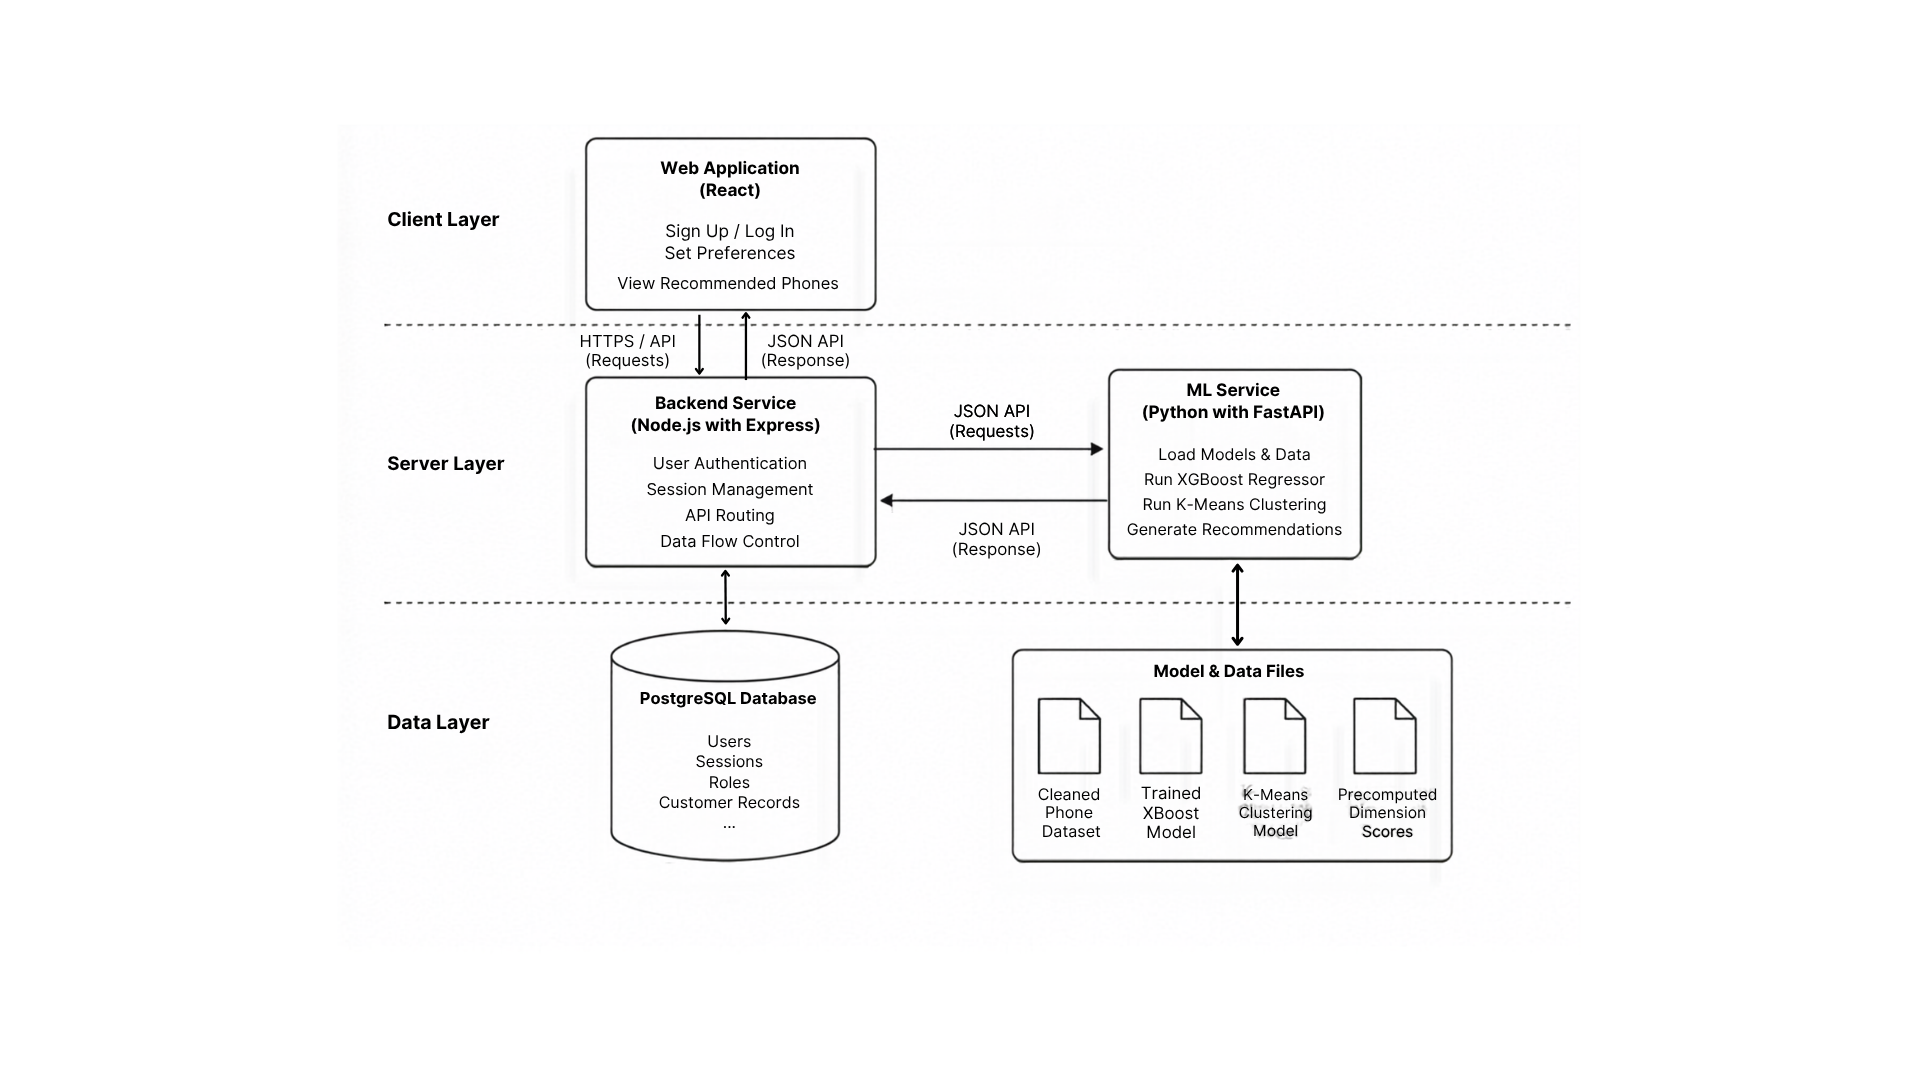
\includegraphics[width=1\textwidth]{Images/sysarch.png}
\caption{System Architecture of the Mobile Recommendation System}
\label{fig:sysarchdesign}
\end{figure}

The system architecture illustrates the layered design of the project, comprising the frontend, backend, database, and machine learning model layers. The frontend is built using React.js and communicates with the backend through REST API endpoints. The backend uses Node.js and Express.js and applies business logic, while the database layer uses PostgreSQL through Prisma ORM. The machine learning layer encapsulates the trained XGBoost model and the K-Means clustering pipeline.

\section{Use Case Diagram}

\begin{figure}[H]
\centering
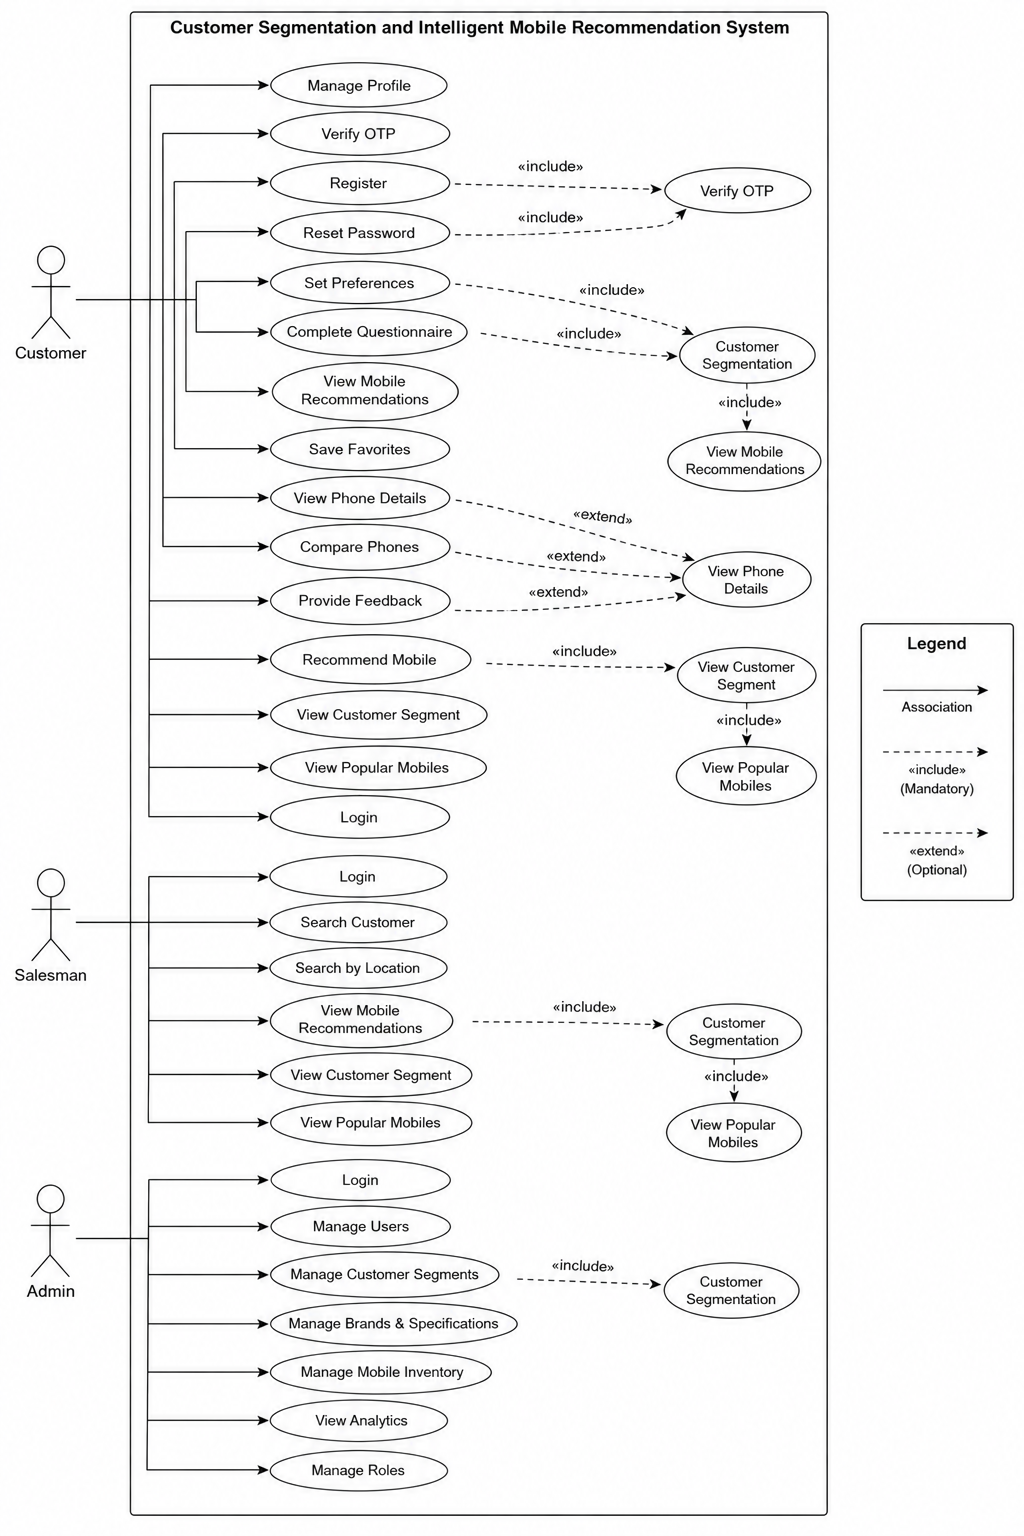
\includegraphics[width=0.95\textwidth]{Images/usecase.png}
\caption{Use Case Diagram of the Mobile Recommendation System}
\label{fig:usecase}
\end{figure}

The use case diagram depicts the three actor roles in the system, namely customer, salesman, and administrator, and the corresponding use cases available to each. The customer can register, log in, set preferences, view recommendations, and view details. The salesman can log in, enter customer details, and view phone recommendations. The administrator can log in, manage users, assign roles, and monitor the system.

\section{Data Flow Diagram}

\begin{figure}[H]
\centering
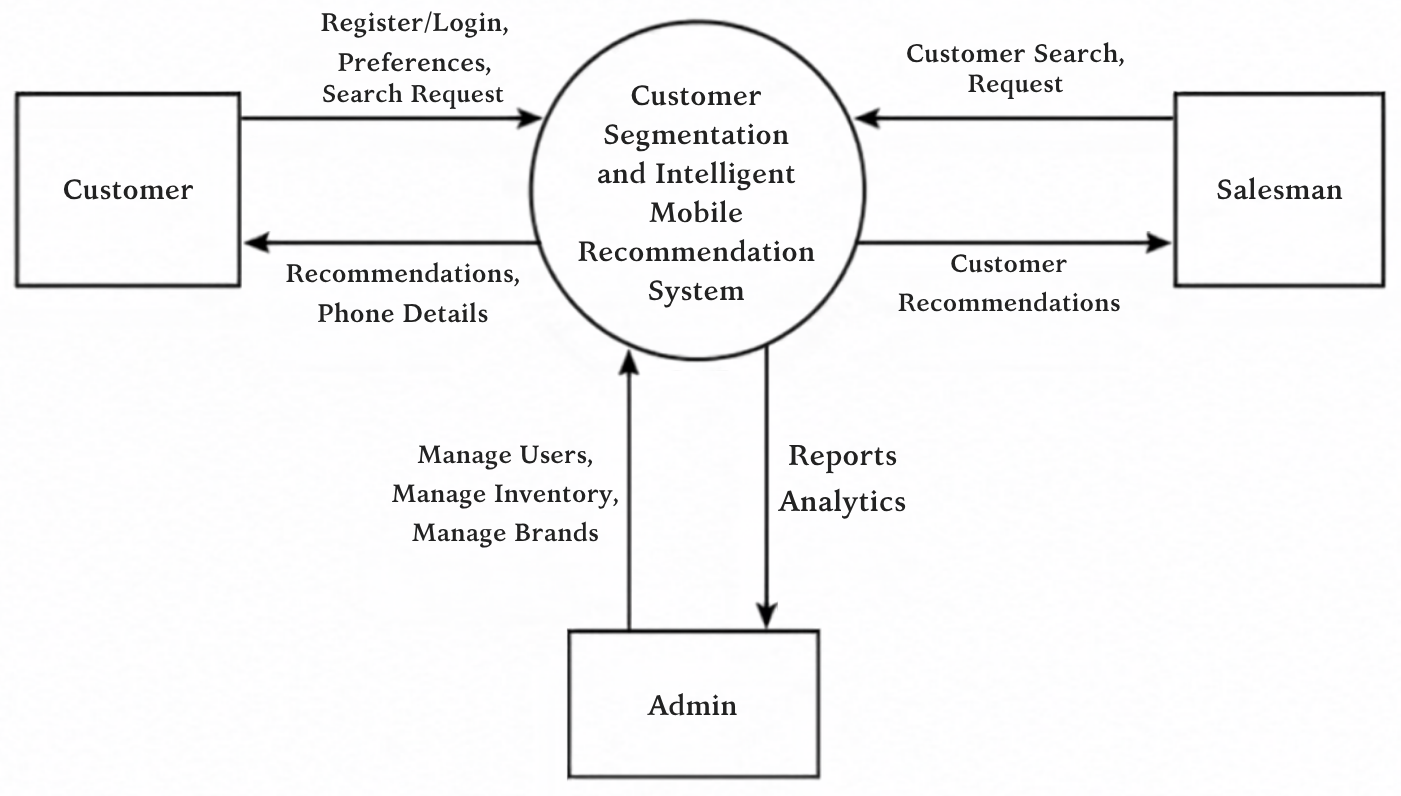
\includegraphics[width=0.95\textwidth]{Images/lvl0dfd.png}
\caption{Level 0 Data Flow Diagram}
\label{fig:lvl0dfd}
\end{figure}

\begin{figure}[H]
\centering
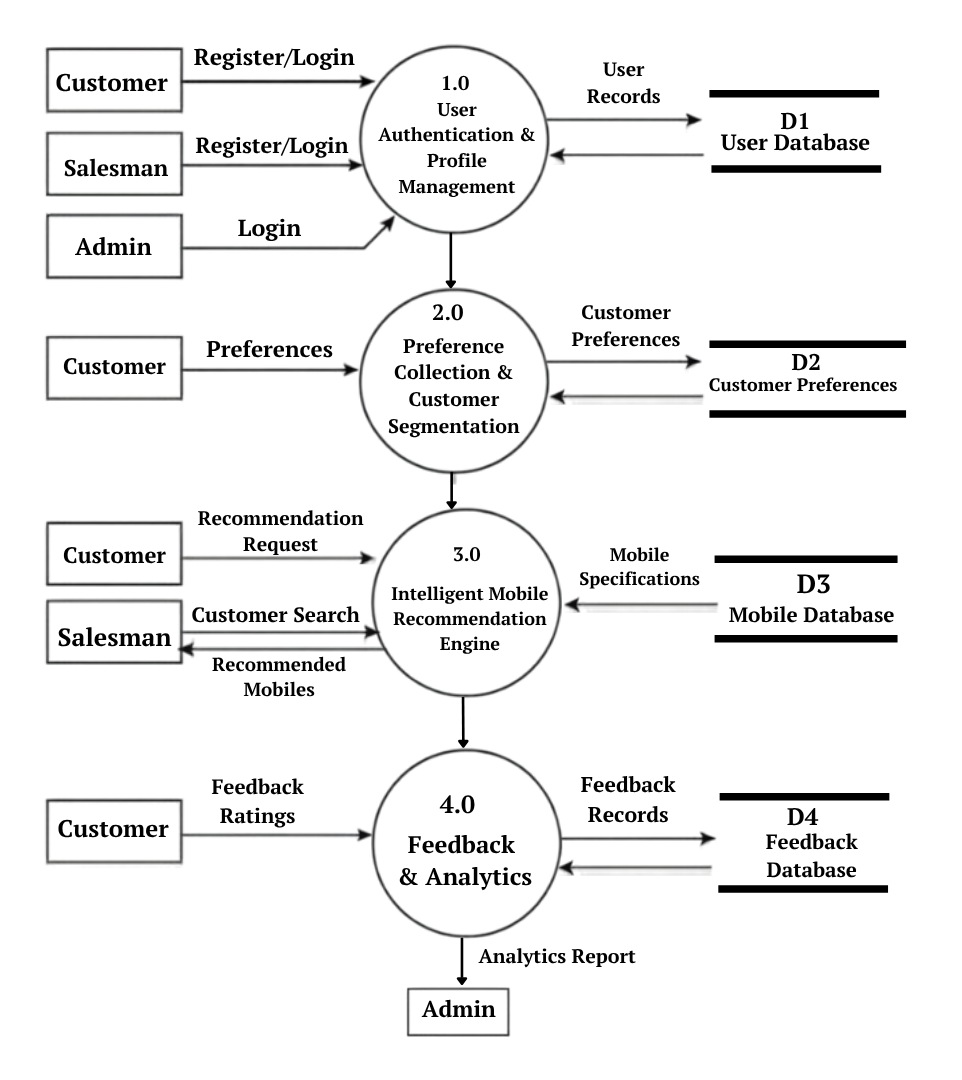
\includegraphics[width=0.95\textwidth]{Images/lvl1dfd.png}
\caption{Level 1 Data Flow Diagram}
\label{fig:lvl1dfd}
\end{figure}

The data flow diagrams describe how information moves between the customer, the system, and the database. At Level 0 the system is shown as a single process that interacts with an external customer and an external database. At Level 1 the internal processes are expanded to show the request handling, machine learning model invocation, and database storage operations.

\section{Iterative Development Model}

\begin{figure}[H]
\centering
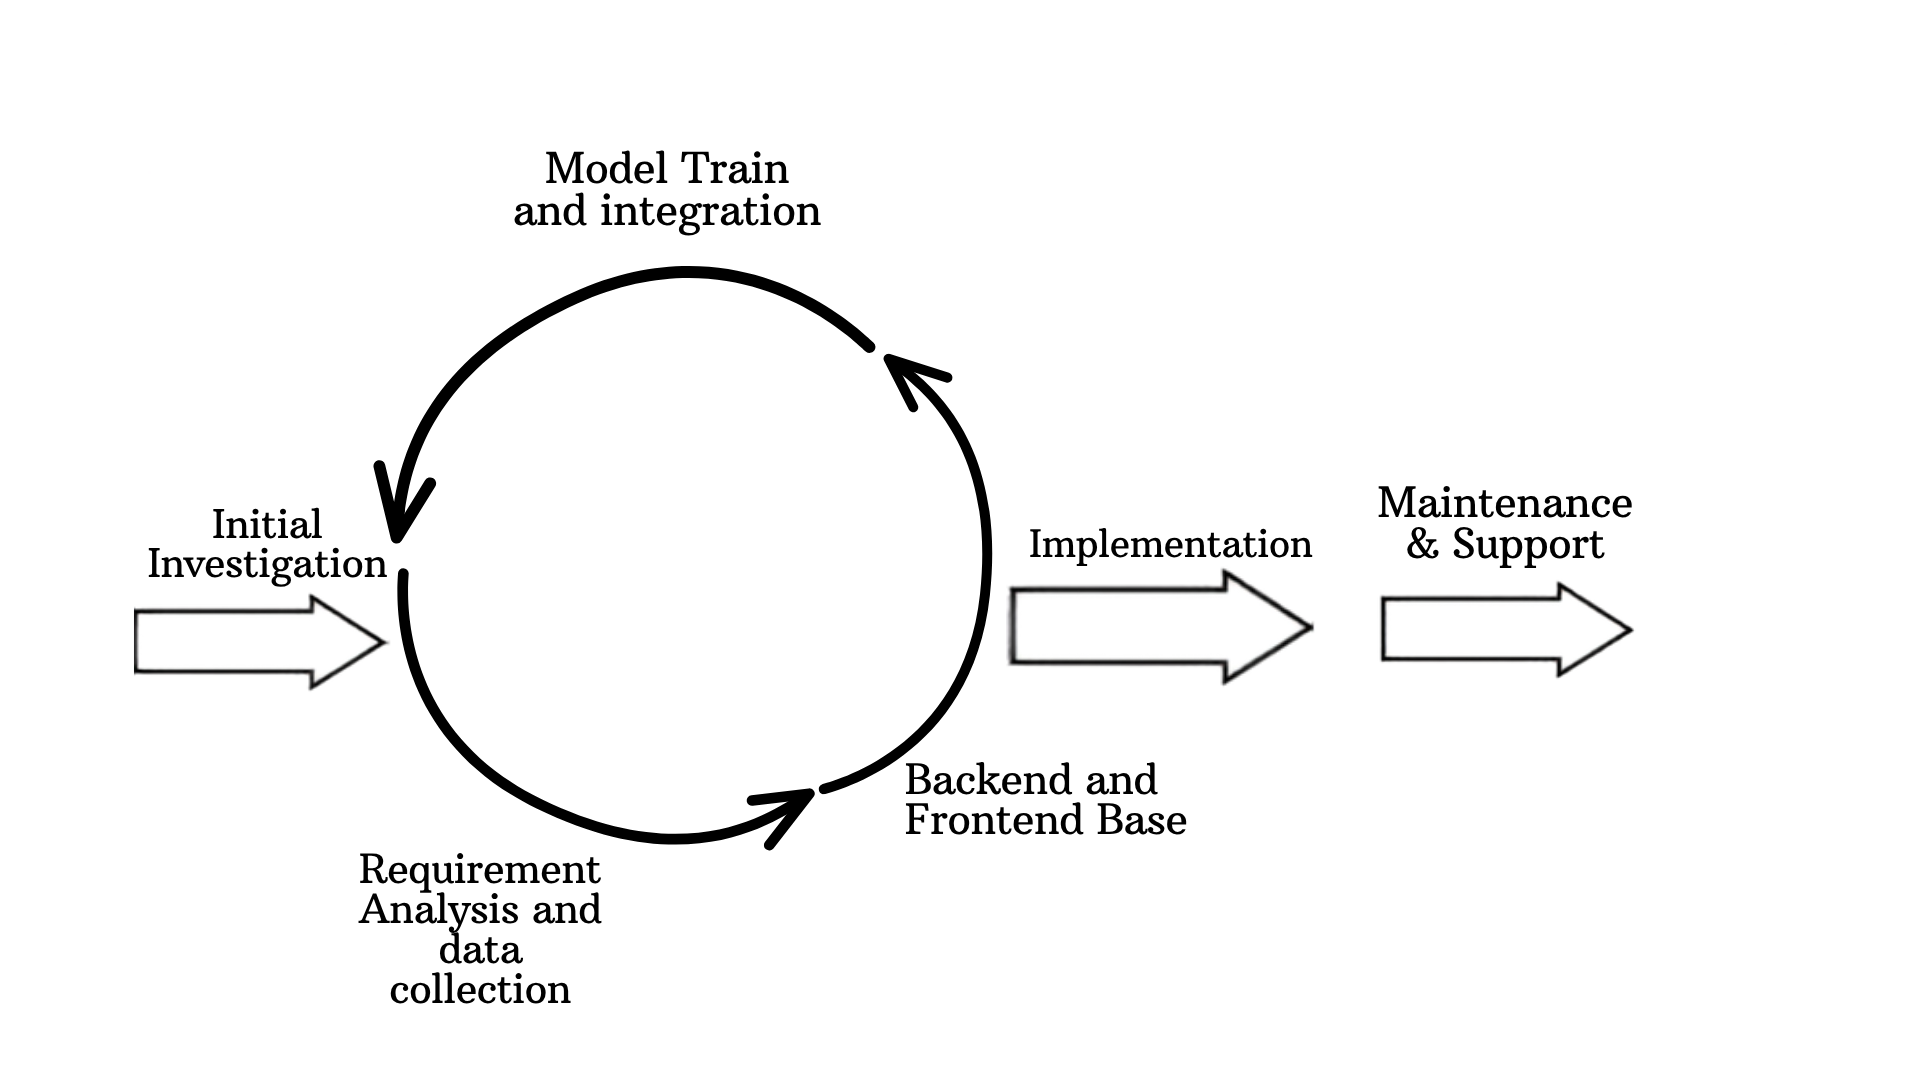
\includegraphics[width=0.9\textwidth]{Images/ITERATIVE_MODEL.png}
\caption{Iterative Development Model}
\label{fig:iterative}
\end{figure}

The project uses an iterative development model in which each iteration refines the previous output. The iterations include requirements gathering, system design, implementation, testing, and review. The model supports continuous improvement and accommodates evolving requirements.

\section{Project Work Plan}

\begin{figure}[H]
\centering
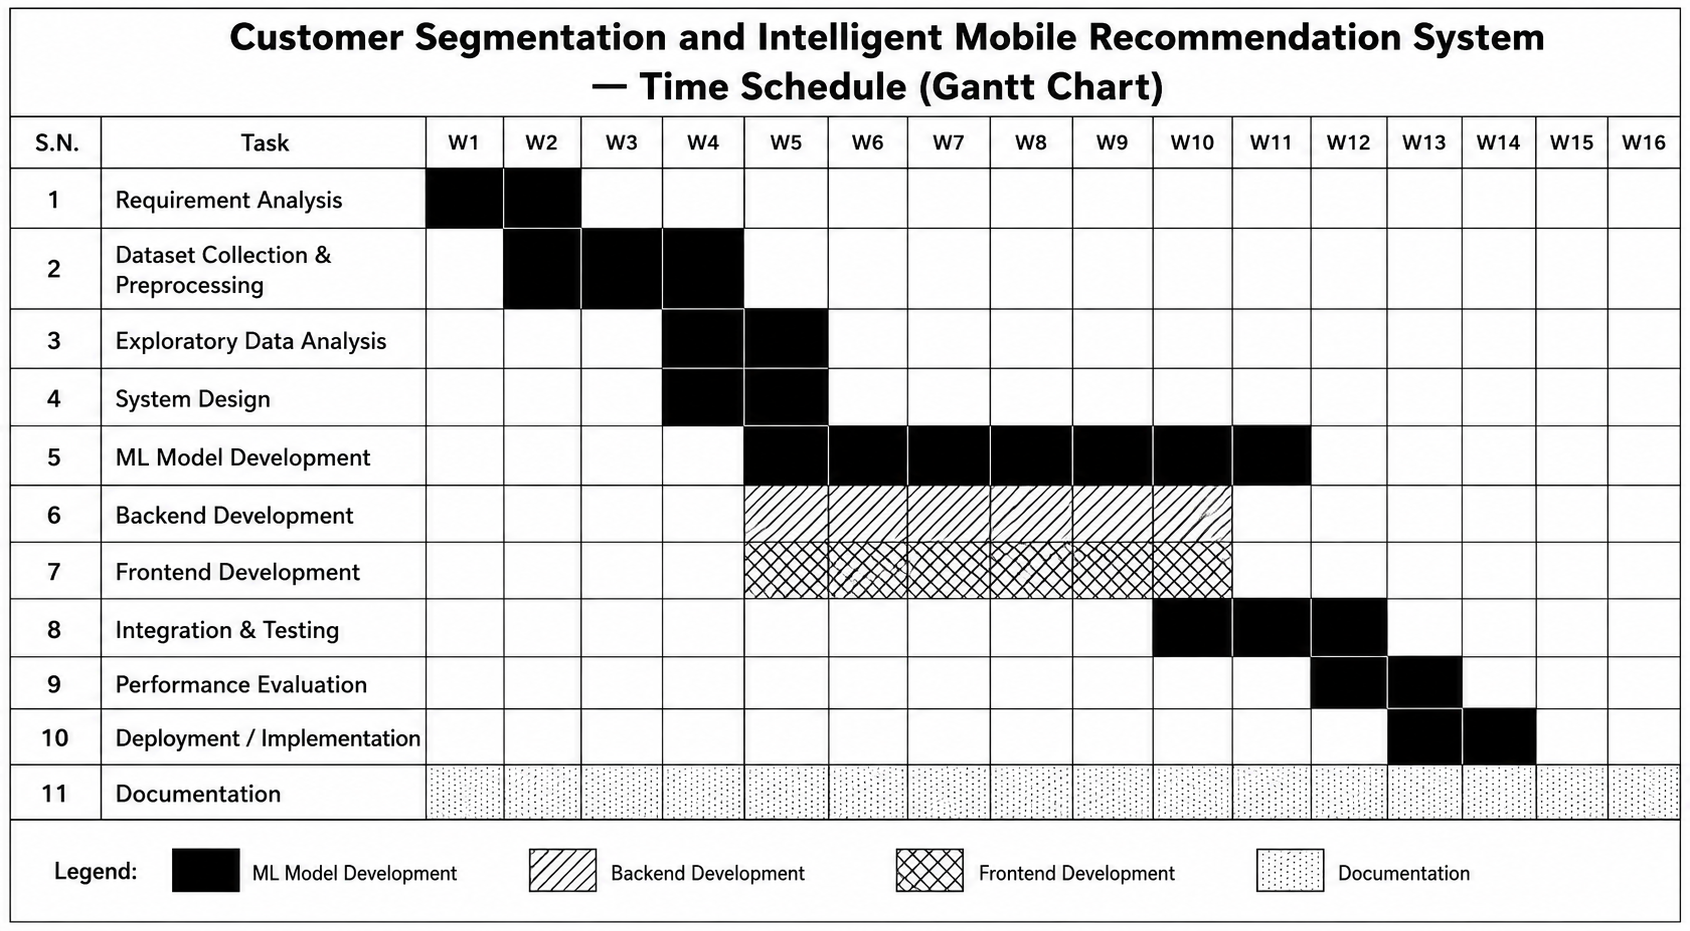
\includegraphics[width=1\textwidth]{Images/Ganttchart.png}
\caption{Gantt Chart of Project Work Plan}
\label{fig:gantt}
\end{figure}

The Gantt chart outlines the timeline of the project activities from data collection and preprocessing through model training, web application development, evaluation, and final report preparation.

\chapter{Results \& Discussion}
This chapter presents the results of the implemented system, the performance of the trained models, and a discussion of the outcome. The results are supported by tables and figures that summarise the experimental findings.

\section{Experiment Setup}

The phone specification dataset and the AnTuTu benchmark scores were collected through web scraping. The customer transaction dataset was synthesised to simulate realistic retail data. The collected data was preprocessed and split into training and test sets in an 80/20 ratio with a fixed random seed. The XGBoost regressor was trained on the log-transformed target and evaluated using 5-fold cross-validation.

\section{Data Preparation Results}

The phone specification dataset and AnTuTu benchmark dataset were successfully collected through web scraping by dividing it into 20 batches and preprocessed. The phone specification and benchmark datasets were merged, while missing values and duplicate records were handled. Feature engineering was performed to prepare the data for machine learning.

\begin{table}[H]
\centering
\caption{Phone Dataset Before Processing}
\label{tab:before-processing}
\begin{tabular}{|l|c|}
\hline
\textbf{Attribute} & \textbf{Value} \\
\hline
Total rows (raw combined batches) & 12,849 \\
\hline
Total columns (raw) & 68 \\
\hline
Columns with $>$55\% missing values & 12 \\
\hline
Exact duplicate rows & 421 \\
\hline
Rows with missing CPU, Chipset and GPU & 1,219 \\
\hline
Missing rate of AnTuTu\_Score & 52.5\% \\
\hline
Missing rate of GeekBench\_Score & 46.1\% \\
\hline
Missing rate of Chipset & 89.6\% \\
\hline
Missing rate of Price\_EUR & 27.2\% \\
\hline
Missing rate of Announced\_Year & 1.1\% \\
\hline
\end{tabular}
\end{table}

Table~\ref{tab:before-processing} shows the state of the raw phone dataset immediately after combining the 20 GSMArena scrape batches, before any cleaning or imputation was applied.

\begin{table}[H]
\centering
\caption{Phone Dataset After Processing}
\label{tab:after-processing}
\begin{tabular}{|l|c|}
\hline
\textbf{Attribute} & \textbf{Value} \\
\hline
Phone specification dataset & 8,500 phones \\
\hline
Phone features after engineering & 152 features \\
\hline
Customer dataset & 4,557 customers \\
\hline
Cities covered & 90 \\
\hline
Exact duplicates removed & 421 rows \\
\hline
Columns dropped ($>$55\% missing) & 12 \\
\hline
Brand names corrected & 596 rows \\
\hline
Missing rate of AnTuTu\_Score & 0.0\% \\
\hline
Missing rate of Chipset & 0.0\% \\
\hline
Missing rate of Price\_EUR & 0.0\% \\
\hline
\end{tabular}
\end{table}

Table~\ref{tab:after-processing} summarises the dataset after all preprocessing, cleaning, and feature engineering steps were completed.

\section{Machine Learning Results}

An XGBoost regression model was trained to predict the AnTuTu performance score from mobile phone specifications. The model achieved satisfactory prediction performance on the test dataset.

\begin{table}[H]
\centering
\caption{XGBoost Model Hyperparameters}
\label{tab:xgb-hyperparams}
\begin{tabular}{|l|c|}
\hline
\textbf{Hyperparameter} & \textbf{Value} \\
\hline
enable\_categorical & True \\
\hline
tree\_method & hist \\
\hline
max\_depth & 10 \\
\hline
min\_child\_weight & 5 \\
\hline
gamma & 0.5 \\
\hline
n\_estimators & 800 \\
\hline
learning\_rate & 0.01 \\
\hline
subsample & 0.7 \\
\hline
colsample\_bytree & 0.7 \\
\hline
reg\_alpha & 1.0 \\
\hline
reg\_lambda & 3.0 \\
\hline
\end{tabular}
\end{table}

The XGBoost model was trained using a set of carefully selected hyperparameters to achieve better predictive performance and generalisation. Table~\ref{tab:xgb-hyperparams} presents the final hyperparameter values used in the model.

\begin{table}[H]
\centering
\caption{XGBoost Training and Testing Performance Metrics}
\label{tab:xgb-performance}
\begin{tabular}{|l|c|c|}
\hline
\textbf{Metric} & \textbf{Training} & \textbf{Testing} \\
\hline
MAE & 0.1416 & 0.1795 \\
\hline
MSE & 0.0507 & 0.0866 \\
\hline
RMSE & 0.2253 & 0.2944 \\
\hline
MAPE & 1.08\% & 1.37\% \\
\hline
RMSLE & 0.0160 & 0.0210 \\
\hline
$R^2$ Score & 0.9241 & 0.8819 \\
\hline
Adjusted $R^2$ & 0.9225 & 0.8707 \\
\hline
\end{tabular}
\end{table}

The performance of the XGBoost model was evaluated on both the training and testing datasets using standard regression metrics. Table~\ref{tab:xgb-performance} compares the training and testing performance, demonstrating the model's ability to generalise well on unseen data.

\begin{table}[H]
\centering
\caption{5-Fold Cross-Validation Results}
\label{tab:xgb-cv-results}
\begin{tabular}{|l|c|}
\hline
\textbf{Metric} & \textbf{Value} \\
\hline
Fold 1 $R^2$ & 0.8824 \\
\hline
Fold 2 $R^2$ & 0.8645 \\
\hline
Fold 3 $R^2$ & 0.8965 \\
\hline
Fold 4 $R^2$ & 0.8912 \\
\hline
Fold 5 $R^2$ & 0.8541 \\
\hline
Mean $R^2$ & 0.8777 \\
\hline
Standard Deviation & 0.0160 \\
\hline
\end{tabular}
\end{table}

To evaluate the stability and generalisation ability of the XGBoost model, 5-fold cross-validation was performed. The R-square scores for each fold, along with the mean and standard deviation, are presented in Table~\ref{tab:xgb-cv-results}.

The obtained results indicate that the model predicts mobile phone performance with good accuracy and generalises well on unseen data.

\begin{figure}[H]
\centering
\begin{minipage}[t]{0.48\textwidth}
    \centering
    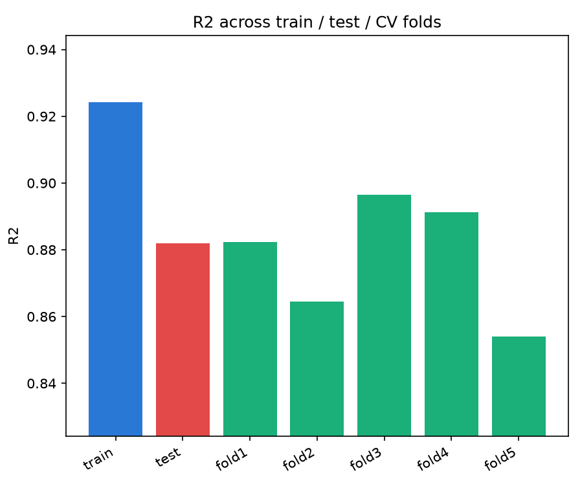
\includegraphics[width=\linewidth]{Images/vis1.png}
    \caption*{$R^2$ Score Validation Plot (Bar Graph)}
\end{minipage}\hfill
\begin{minipage}[t]{0.48\textwidth}
    \centering
    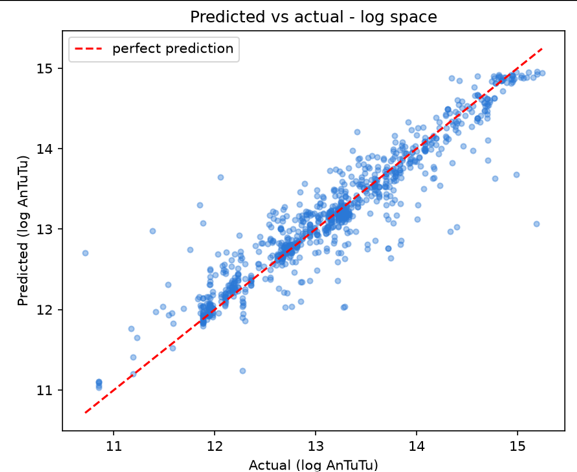
\includegraphics[width=\linewidth]{Images/vis2.png}
    \caption*{Predicted vs. Actual Plot for Log AnTuTu}
\end{minipage}

\vspace{0.5em}

\begin{minipage}[t]{0.48\textwidth}
    \centering
    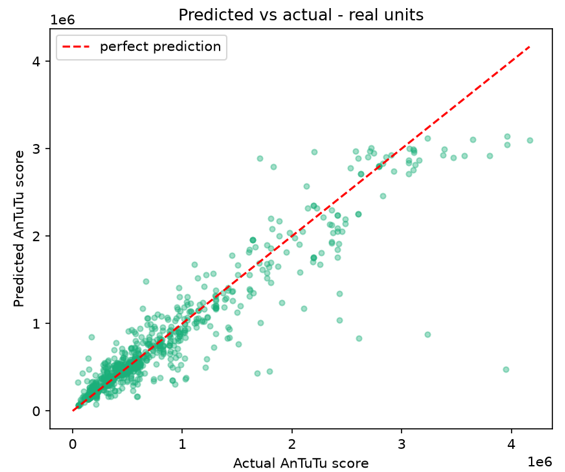
\includegraphics[width=\linewidth]{Images/vis3.png}
    \caption*{Predicted vs. Actual Plot for Real Units AnTuTu}
\end{minipage}\hfill
\begin{minipage}[t]{0.48\textwidth}
    \centering
    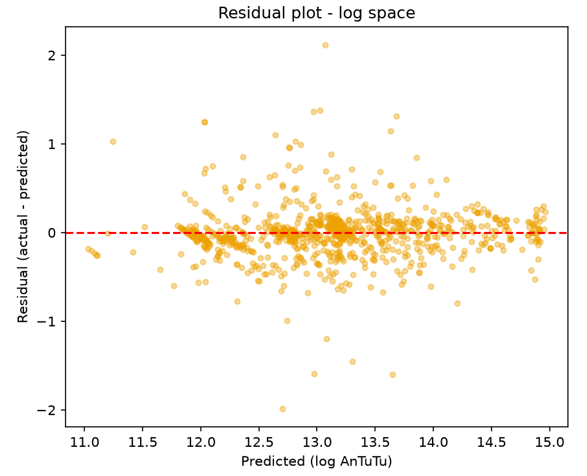
\includegraphics[width=\linewidth]{Images/vis4.png}
    \caption*{Predicted vs Actual Residual plot}
\end{minipage}
\caption{Visualizations of XGBoost Regressor Performance on the Test Set}
\label{fig:visuals}
\end{figure}

To better understand the model's performance, several visualisations were generated from the trained XGBoost regressor. The predicted versus actual score plot shows that most predictions lie close to the diagonal line, indicating good accuracy. The error distribution is centred around zero, suggesting minimal prediction bias. The feature importance plot highlights the phone specifications that contribute most to the predicted AnTuTu score. Together, these visualisations support the strong performance metrics reported in the table.

\begin{figure}[H]
\centering
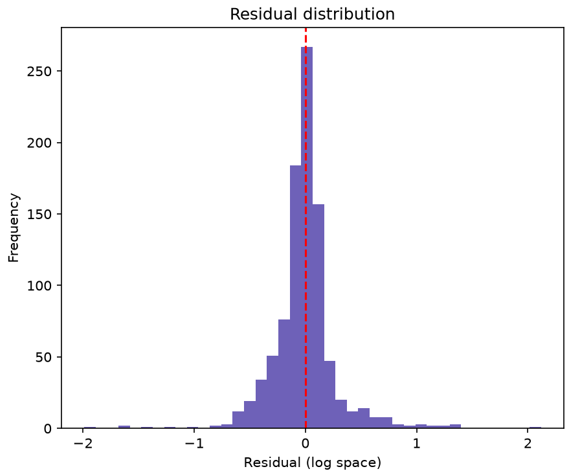
\includegraphics[width=0.9\textwidth]{Images/vis5.png}
\caption{SHAP Feature Importance Summary Plot}
\label{fig:shap}
\end{figure}

The SHAP summary plot highlights the most influential phone features driving the predictions of the XGBoost model.

\section{Recommendation System Output}
The recommendation system was successfully implemented. The current system is capable of predicting the AnTuTu performance score of a phone, generating personalised phone recommendations, ranking recommended phones based on user preferences, and explaining prediction results using SHAP feature importance.

\section{Software Development Approach}

The web application was developed using an iterative development model. Each iteration added a new feature or refined an existing one based on testing and feedback. The backend was first implemented with RESTful endpoints, the database schema, and the authentication flow. The frontend was then connected through API integration, and the machine learning models were deployed through the backend.

\section{Model Deployment}

The trained XGBoost model and K-Means pipeline are serialised to disk as Python pickle files and loaded by the backend at startup. The Python machine learning service is invoked through a thin Node.js wrapper that calls a Python interpreter script for inference. This avoids embedding Python in the Node.js process while keeping the inference latency low.

\section{User Interface and Backend}

The backend has been developed using Node.js, Express.js, PostgreSQL, and Prisma ORM. Authentication features including user registration, login, OTP verification, password reset, and session management have been completed.

The frontend has been developed using React and currently includes: User Login Page, Registration Page, OTP Verification Page, Password Reset Page, and the Dashboard User Interface.

\begin{figure}[H]
\centering
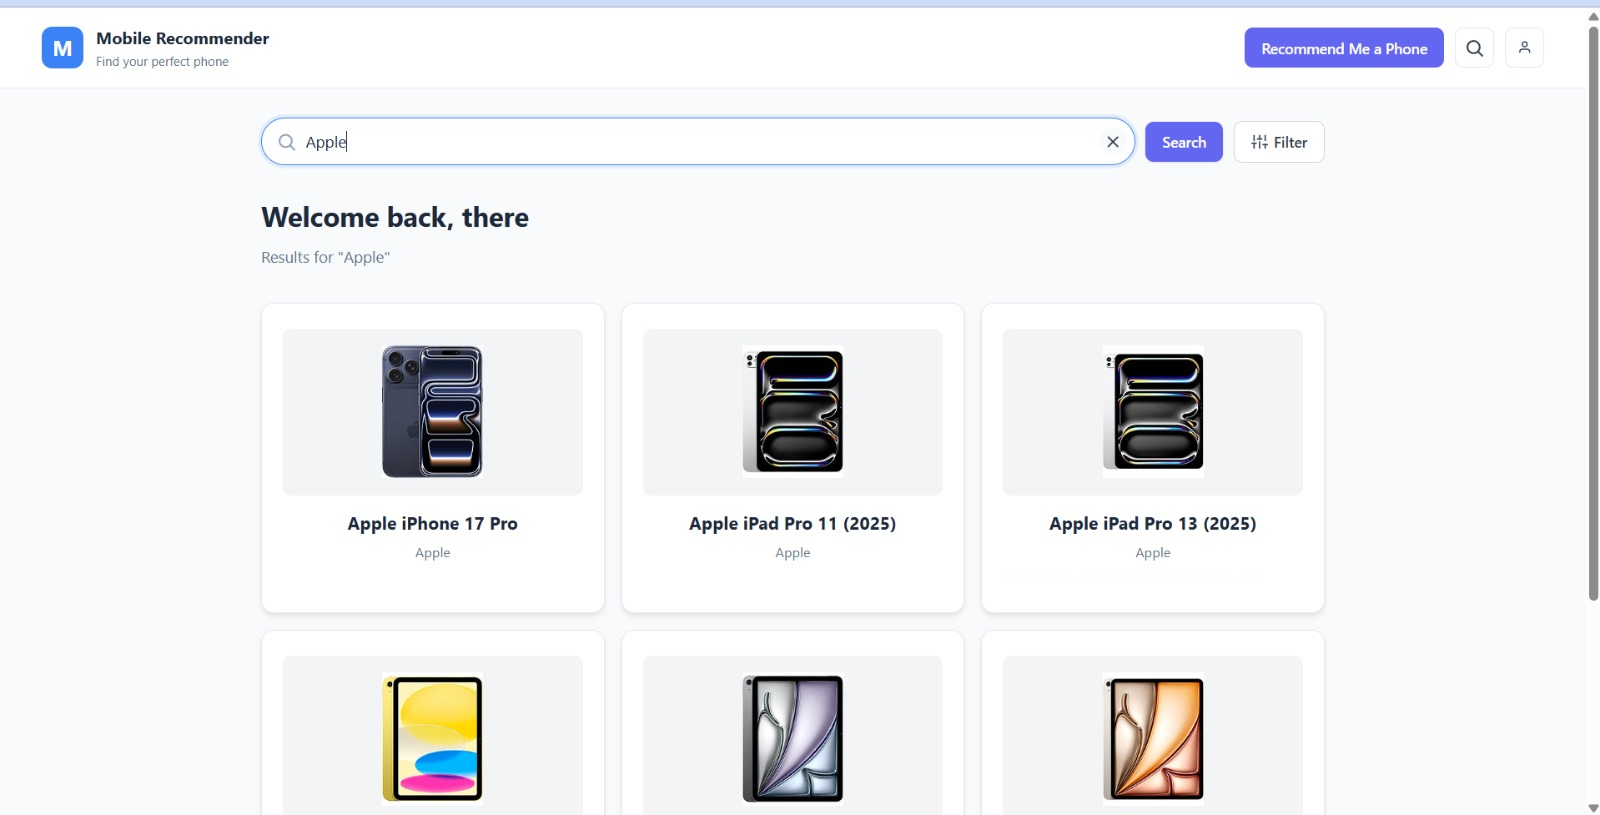
\includegraphics[width=0.9\textwidth]{Images/frontendui.jpeg}
\caption{Frontend User Interface of the Mobile Recommendation System}
\label{fig:frontendui}
\end{figure}

The machine learning, frontend, and backend components have been integrated for simple recommendation generation based on user preferences.

\section{Testing, Evaluation, and Validation}

The system was tested in two stages. The first stage validated the trained models on a held-out 20\% test split using regression and clustering metrics, as shown in Tables~\ref{tab:xgb-performance} and~\ref{tab:xgb-cv-results}. The second stage validated the integrated web application through end-to-end tests that mimic the actual user workflow: a customer registers, logs in, sets preferences, and views recommended phones; a salesman enters customer details and views phone recommendations; and an administrator manages users and views monitoring information.

\chapter{Conclusions}
This project successfully demonstrated a complete machine learning based mobile recommendation system that combines customer segmentation with hardware-aware phone scoring. The proposed pipeline integrates web scraping, data preprocessing, feature engineering, XGBoost regression, K-Means clustering, SHAP-based explainability, and a full-stack web application behind a single end-to-end system.

The XGBoost regressor achieved an R\textsuperscript{2} score of approximately 0.88 on the held-out test set with a mean absolute error of 0.18 in log-space, indicating that the model predicts the benchmark score of mobile phones with high accuracy. The 5-fold cross-validation produced a mean R\textsuperscript{2} of 0.88 with a low standard deviation, which confirms that the model generalises well and is not overfitting to the training data. The K-Means clustering pipeline grouped customers into segments with a strong silhouette score, allowing the recommendation engine to apply segment-specific ranking strategies. The integration of SHAP makes the predictions of the XGBoost model transparent by quantifying the contribution of each phone feature, which is essential for building user trust.

The web application fulfils all functional and non-functional requirements set out in the system design chapter. Customers can register, log in, set preferences, and view recommended phones. Sales staff can enter customer details and receive ranked recommendations. Administrators can manage users and monitor activity. The use of PostgreSQL through Prisma ORM provides a robust and maintainable data layer.

Overall, the project demonstrates that combining a gradient boosting regressor with a clustering-based segmentation pipeline and an explainability layer produces useful, interpretable, and actionable recommendations for mobile phone retailers. The architecture is modular and extensible, which supports future iterations to improve recommendation quality and to incorporate new data sources.

\chapter{Limitations and Future Enhancement}
This chapter describes the major limitations of the project and the further enhancements that can be incorporated into the system.

\section{Limitations}

\begin{enumerate}
    \item The customer transaction dataset is synthetic and does not capture the full noise and distribution of real retailer data.
    \item The recommendation engine is a ranker that uses hard filters and a weighted sum of dimension scores; it does not learn from interaction history through collaborative filtering.
    \item The benchmark coverage on GSMArena and AnTuTu is incomplete, with missing values for many older or less popular phones.
    \item The model is a single XGBoost regressor and does not account for time-based changes in customer preferences.
    \item The deployed system does not perform real-time incremental updates; the model is refit offline.
\end{enumerate}

\section{Future Enhancement}

\begin{enumerate}
    \item Incorporate collaborative filtering and matrix factorisation alongside content-based ranking to address the cold-start problem more comprehensively.
    \item Replace the synthetic customer dataset with real retailer data (subject to appropriate consent and privacy controls).
    \item Add a temporal component to capture changes in customer preferences and product releases over time.
    \item Deploy the system on a containerised platform such as Docker and Kubernetes to simplify scaling.
    \item Add A/B testing infrastructure to evaluate the impact of the recommendation system on customer behaviour in production.
\end{enumerate}

\addcontentsline{toc}{section}{References}
\renewcommand{\bibname}{References}
\bibliographystyle{unsrt}
\bibliography{ref}
\chapter*{Appendices}
\addcontentsline{toc}{section}{Appendices}
The following appendices provide supplementary information about the project including the architecture diagrams, workflow descriptions, and project planning notes that supported the implementation.

\section*{Appendix A: System Architecture Overview}
Content to be added.

\section*{Appendix B: ML Workflow Details}
Content to be added.

\section*{Appendix C: Project Planning Notes}
Content to be added.

\end{document}
